
% ===========================
\chapter{Grundlagen}
\label{grundlagen}
% ===========================

In diesem Kapitel werden die zum Verständnis nötigen Grundlagen für diese Arbeit erklärt. Dabei wird im Abschnitt \ref{grundlagen_fahren} der Stand der Technik von automatisierten Fahrfunktionen und deren Entwicklung beschrieben. Im Abschnitt \ref{grundlagen_nn} wird maschinelles Lernen im Allgemeinen und im Speziellen \acp{KNN}, die für die Umsetzung dieser Arbeit nötig sind, beschrieben.

% ===========================
\section{Hochautomatisiertes Fahren}
\label{grundlagen_fahren}
% ===========================

Hochautomatisiertes Fahren wird in den vergangenen Jahren zunehmend von der Automobilindustrie vorangetrieben. Aktuelle \ac{FAS}, wie der Spurhalteassistant oder die Abstandsregelung, sind nach der Norm SAE J3016 (Abbildung \ref{fig_level_autonomes_fahren}) bei Level 2 des autonomen Fahrens eingeordnet. Dabei kontrolliert stets der Fahrer die Funktion des Assistenzsystems und überwacht die Umgebung. Ab Stufe 3 des autonomen Fahrens kontrolliert das System die Umgebung und die Funktion der \ac{FAS} \cite{sae2014taxonomy}. Die Kontrollinstanz des Fahrers existiert nicht mehr und die Sicherheit von Fahrfunktionen muss in jedem potentiellen Szenario garantiert sein. Das betrifft sowohl alle bekannten Szenarien, als auch alle bisher unbekannten Szenarien. Da für zukünftige \ac{FAS} nicht mehr alle Szenarien bekannt sind, kann die Absicherung der Funktionen nicht garantiert werden. Das stellt Automobilhersteller und Automobilzulieferer vor große Herausforderungen.

%Das schließt sowohl die Entwicklung von \ac{FAS} als auch die dazu benötigten Testszenarien ein \cite{pfeffer2016continuous}.

In den folgenden Abschnitten wird erläutert, wie aktuell diesen Herausforderungen begegnet wird. In Abschnitt \ref{grundlagen_fahren_entwicklung} wird ein allgemeiner Überblick über die aktuellen Entwicklungsmethodiken für \ac{FAS} gegeben. Danach werden in Abschnitt \ref{grundlagen_fahren_szenarien} bisherige Ansätze für die Klassifizierung von Fahrszenarien vorgestellt.

\begin{figure}[h]
\centering
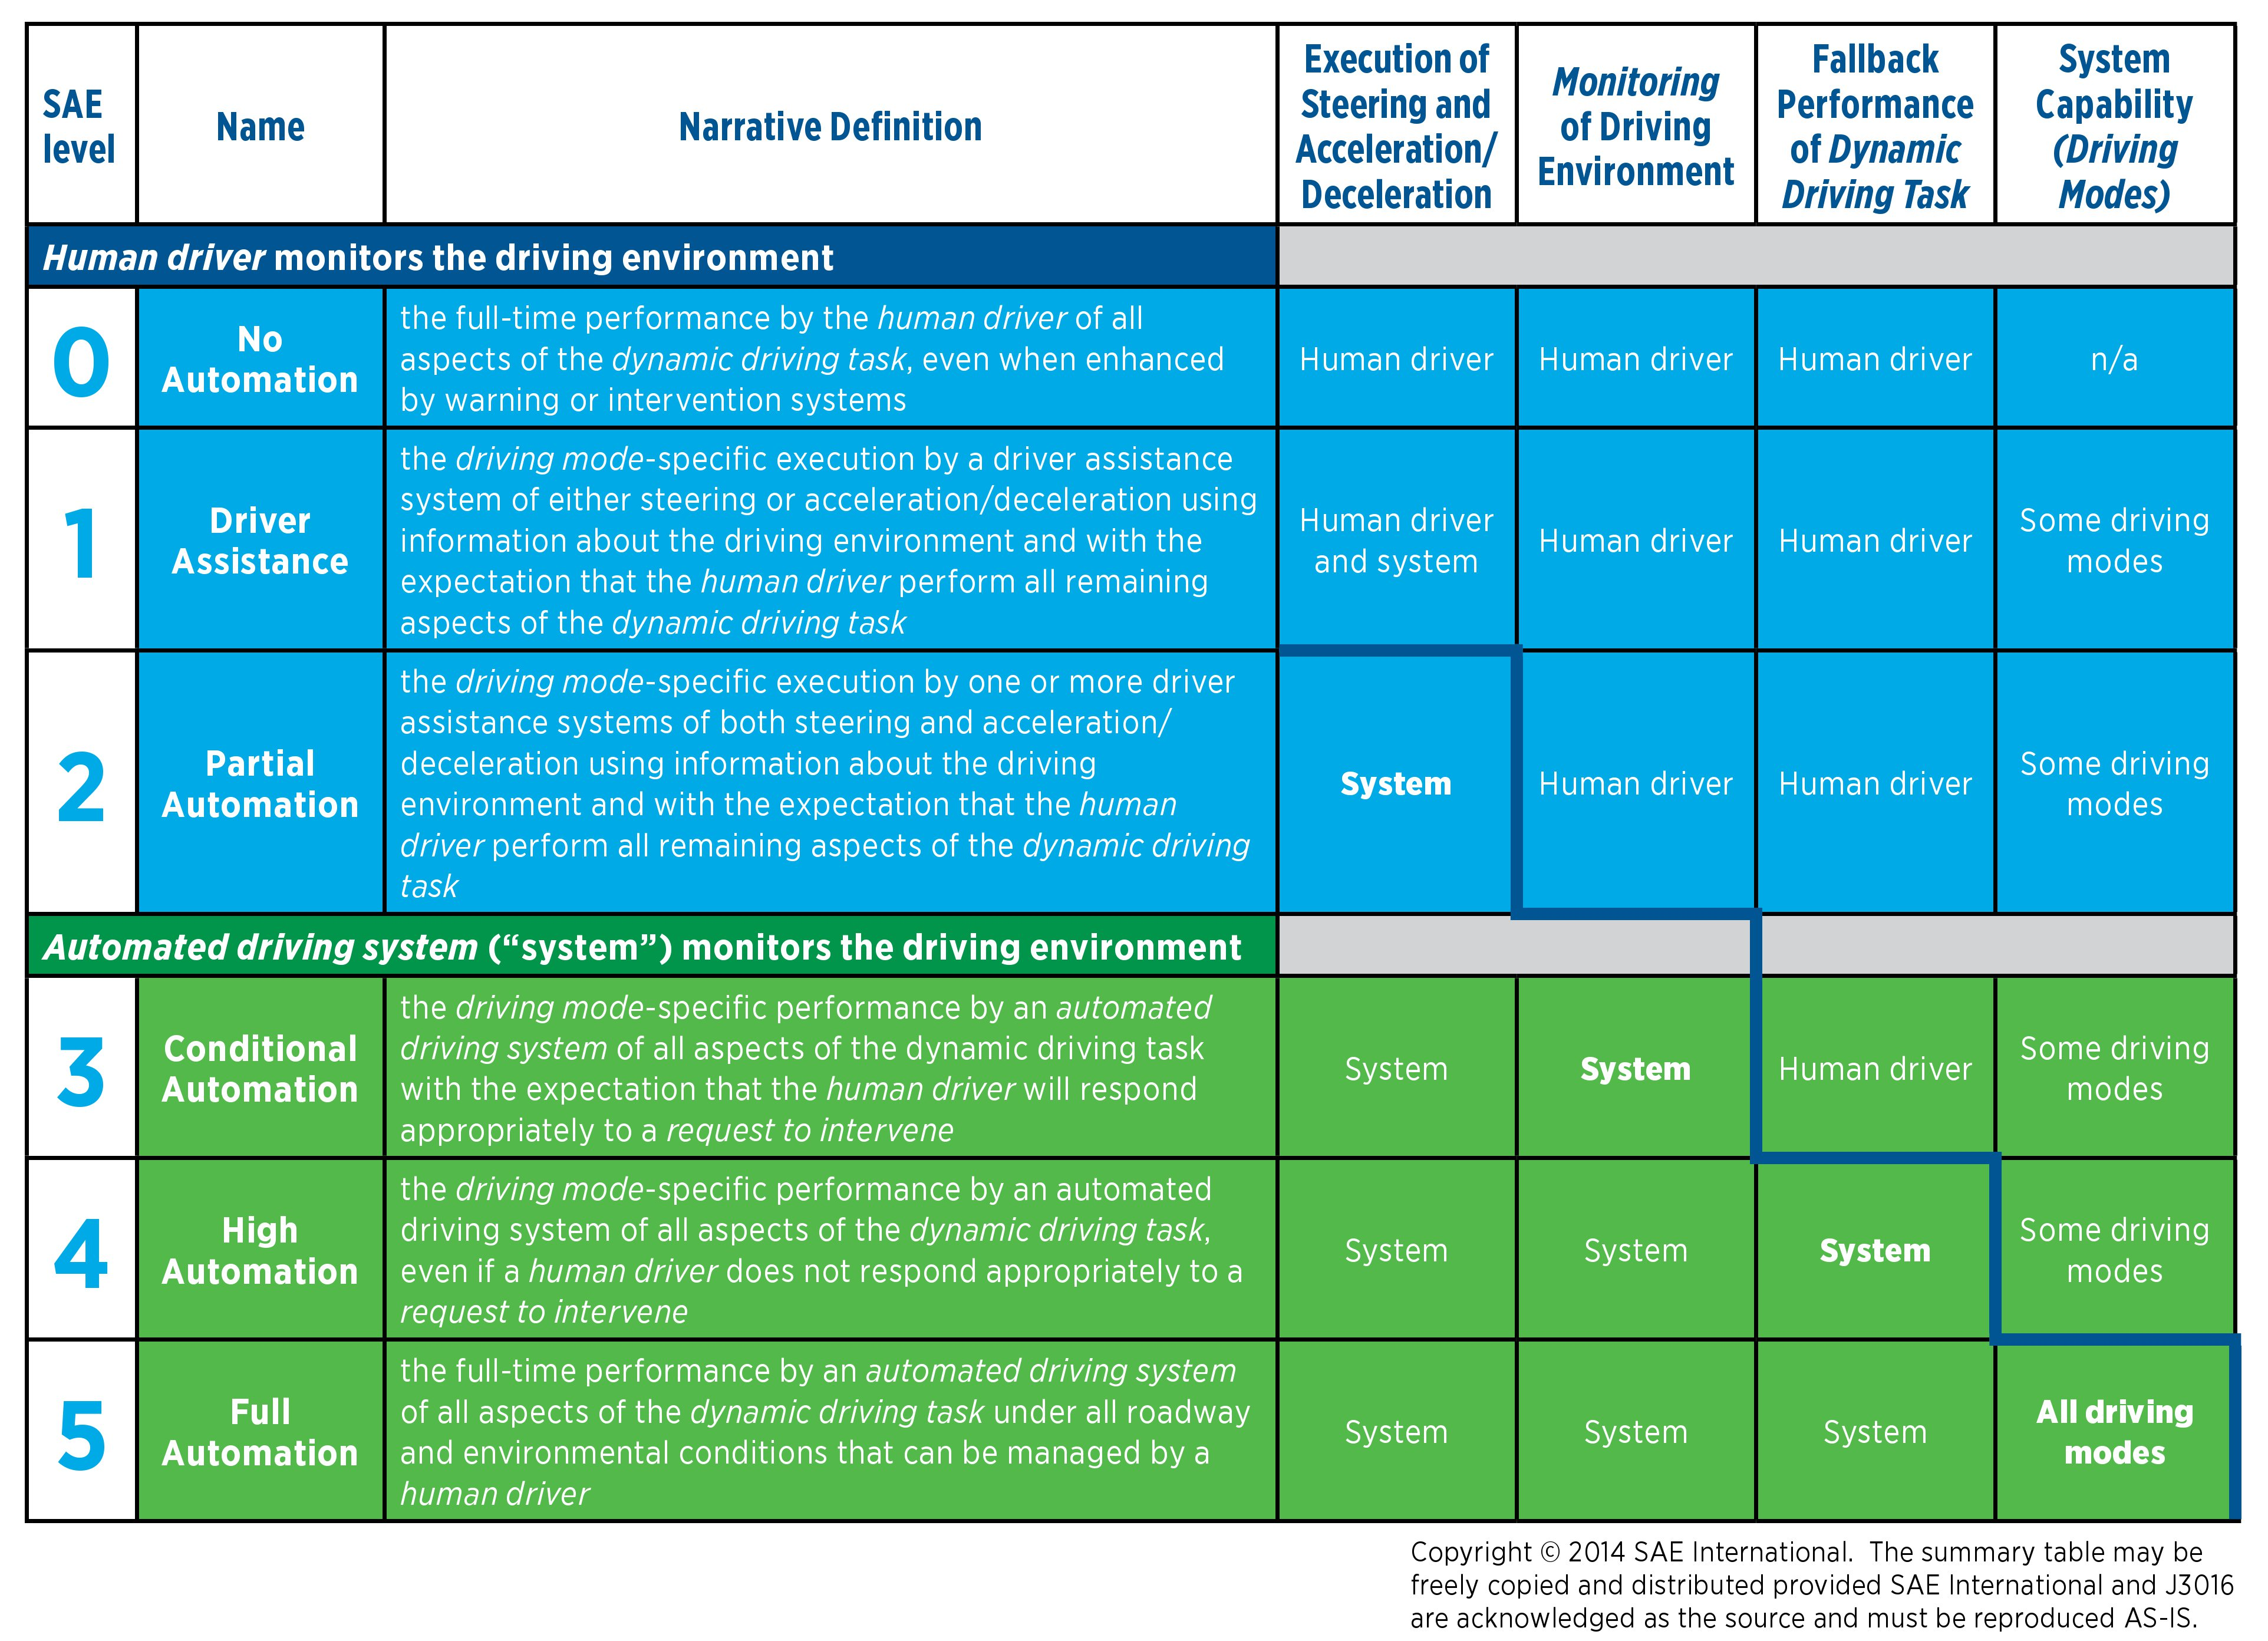
\includegraphics[scale=0.7]{images/level_autonomes_fahren.jpg}
\caption[Norm SAE J3016 für die Stufen des autonomen Fahrens]{Norm SAE J3016 für die Stufen des autonomen Fahrens, entnommen aus \cite{sae2014taxonomy}}
\label{fig_level_autonomes_fahren}
\end{figure}


% ===========================
\subsection{Entwicklung von Fahrerassistenzfunktionen}
\label{grundlagen_fahren_entwicklung}
% ===========================

\ac{FAS} sind Funktionen im Kraftfahrzeug, die den Fahrer unterstützen. Diese Systeme nutzen Sensordaten, wie Radar-, Ultraschall-, oder Kameradaten, aus dem Fahrzeug, um den Fahrer dann auf Basis der abgeleiteten Informationen zu unterstützen. Beispielsweise erkennt ein Spurhalteassistent wenn das Fahrzeug die Spur verlässt und kann die Fahrlinie korrigieren. 

Um \ac{FAS} effizient zu entwickeln und schon früh einzelne Komponenten testen zu können, werde diese in der Automobilindustrie häufig mit dem V-Modell als Vorgehensmodell entwickelt. Damit soll die Planungssicherheit und die Qualität der Entwicklung erhöht werden. Das V-Modell ist ein chronologisches Vorgehensmodell und aus der Softwareentwicklung adaptiert \cite{vmodell2005}. Das V-Modell kann in einen linken absteigenden und einen rechten aufsteigenden Ast unterteilt werden. Der linke Ast enthält die Funktionsanforderungen, die nach unten weiter detailliert und aufgeschlüsselt werden. Der rechte Ast umfasst aufsteigend Funktionstests auf dem jeweiligen Detaillierungsgrad \cite{hakuli2015virtuelle}. Das V-Modell ist in einer einfachen Version in Abbildung \ref{fig_v_modell} dargestellt.

\begin{figure}[h]
\centering
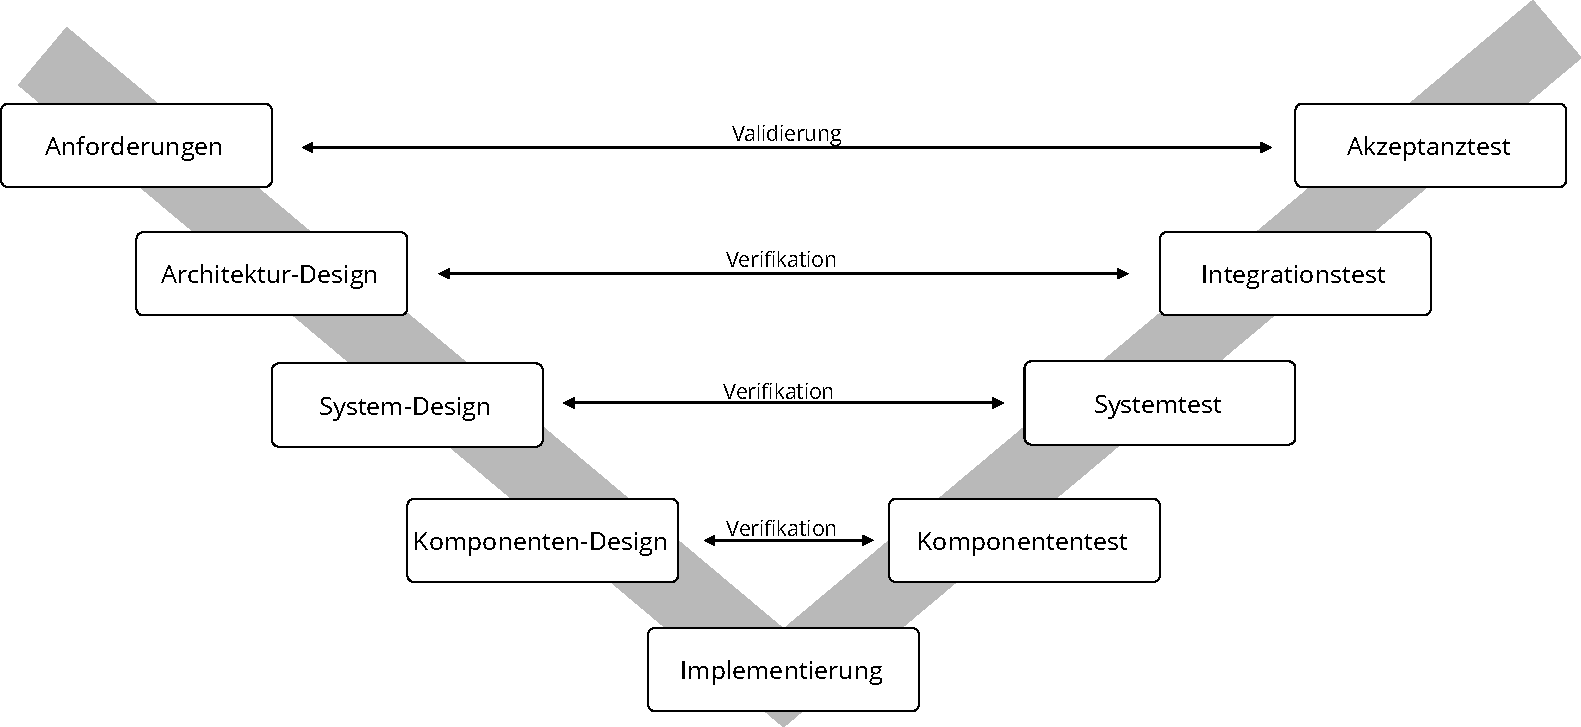
\includegraphics[scale=0.5]{images/v_modell.pdf}
\caption[V-Modell]{V-Modell \cite{hakuli2015virtuelle}}
\label{fig_v_modell}
\end{figure}

Die Schritte auf dem absteigenden und aufsteigenden Ast haben jeweils eine Beziehung. Jeder Test auf dem aufsteigenden Ast verifiziert bzw. validiert den dazugehörigen Entwicklungsschritt auf dem absteigenden Ast. Dementsprechend werden oben im V-Modell die Kundenanforderungen auf dem absteigenden Ast erfasst und auf dem aufsteigenden Ast validiert. Unten im V-Modell werden einzelne Hardware- oder Softwarekomponenten entwickelt, die die entsprechenden Kundenanforderungen von oben lösen sollen. Diese werden anschließend auf dem aufsteigenden Ast verifiziert \cite{hakuli2015virtuelle}.

% ===========================
\subsubsection{Testfälle für die Validierung und Verifikation}
% ===========================

Die Validierung und Verifikation von \ac{FAS} folgt dem Testkonzept. Ein Testkonzept umfasst die Analyse des Testobjektes, die Generierung von Testfällen, die Durchführung von Tests und schließlich die Testauswertung \cite{schuldt2013effiziente}. Diese Schritte sind in der Abbildung \ref{fig_testfallerstellung} dargestellt.

\begin{figure}[h]
\centering
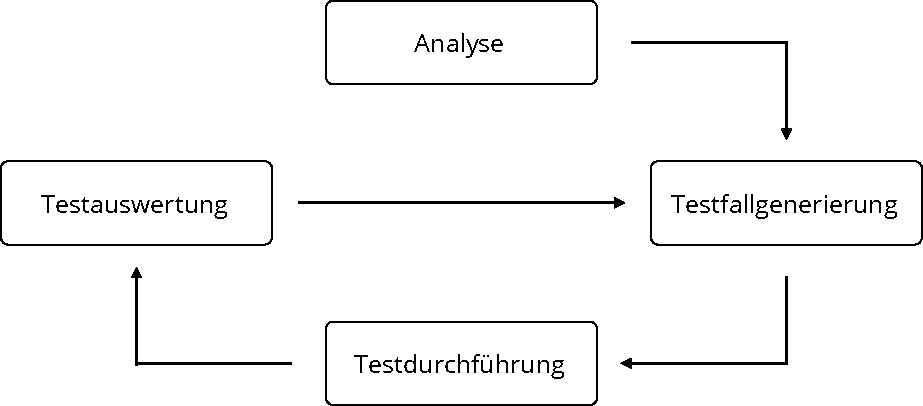
\includegraphics[scale=0.7]{images/testfallerstellung.pdf}
\caption[Schritte zur Testfallerstellung]{Schritte zur Testfallerstellung \cite{schuldt2013effiziente}}
\label{fig_testfallerstellung}
\end{figure}

Testfälle werden bereits möglichst früh im Entwicklungsprozess erstellt, um eine hohe Qualität von \ac{FAS} und einzelnen Komponenten zu erreichen \cite{wachenfeld2015freigabe}. Hierfür werden in der Praxis virtuelle Fahrversuche eingesetzt. Die Idee ist eine stufenweise Digitalisierung von Komponenten aus dem realen Fahrversuch mit den Zielen die Reproduzierbarkeit zu steigern, den Aufwand zu reduzieren und insgesamt flexibler zu werden. Im virtuellen Fahrversuch werden in der frühen Konzeptphase alle Komponenten virtuell getestet und dann schrittweise durch Hardwarekomponenten ersetzt. Schließlich werden alle Komponenten im realen Fahrversuch auf der Straße mit einem realem Fahrer und anderen Verkehrsteilnehmern getestet \cite{hakuli2015virtuelle}.

Beim virtuellen Fahrversuch spielen die Konzepte \ac{MiL}, \ac{SiL}, \ac{HiL} und \ac{ViL} eine wichtige Rolle. Mit \ac{MiL} und \ac{SiL} werden Funktionen auf Basis von Simulationsmodellen getestet \cite{berg2015vehicle}, indem Hardwarekomponenten simuliert werden. Mit fortschreitender Entwicklung werden immer mehr Simulationskomponenten durch die entsprechende Hardware ersetzt und mit \ac{HiL} getestet \cite{hakuli2015virtuelle}. \ac{ViL} schließt schließlich die Lücke zwischen virtuellem Fahrversuch und realem Fahrversuch. Dieses Testkonzept macht die Komplexität bei der Entwicklung von \ac{FAS} beherrschbar und reduziert den Testaufwand \cite{schwab2014durchgangige}. Für die Freigabe von \ac{FAS} ist die Realfahrt die wichtigste Methode, da sie aktuell die beste Validierung bei annehmbaren ökonomischen Aufwand ist \cite{wachenfeld2015freigabe}.

Mit steigender Automatisierung von \ac{FAS} steigt auch die Anzahl möglicher Szenarien, in denen die Sicherheit der Funktionen auch ohne Fahrer garantiert sein muss. Um alle Funktionen ausreichend testen zu können, steigt die Anzahl der benötigten Testfälle. Testfälle müssen alle potentiell eintretenden Szenarien, in denen das \ac{FAS} zum Einsatz kommen kann, abdecken. Dadurch steigt mit hochautomatisierten Funktionen der Aufwand für Validierung und Verifikation mit Testfällen \cite{bach2017reactive}. Eine Möglichkeit für die Reduzierung von Testfällen ist es, kritische Situationen zu finden und Testfälle mit weniger kritischen Situationen zu entfernen \cite{wachenfeld2015freigabe}.

Heute werden Testfälle auf der Basis von Anforderungen an die Fahrfunktionen und Standardsituationen abgeleitet und getestet. Dabei wächst heute schon, mit der Beschränkung auf Standardfälle, der Testaufwand \cite{surmund2018neue}. Mit zukünftigen hochautomatisierten \ac{FAS} ab Stufe 3 des autonomen Fahrens muss das System in allen potentiellen Szenarien sicher sein und Testfälle dürfen nicht mehr auf die Standardsituationen begrenzt sein. Die Sicherheit des Gesamtsystems muss in breiterem Spektrum mit einer Vielzahl Szenarien ohne Eingriff des Fahrers garantiert werden können. Das bedeutet, dass die bisherigen Standardsituationen um neue Szenarien erweitert werden müssen \cite{surmund2018neue}.

Für die Erstellung von Testfällen müssen daher alle potentiell eintretenden kritischen Szenarien bekannt sein. Der Ansatz in dieser Arbeit ist es, bekannte Szenarien zu klassifizieren und auf diese Weise bisher unbekannte und möglicherweise kritische Szenarien zu finden. Dies soll mit Hilfe von simulierten Daten geschehen, um die Skalierbarkeit mit angemessenem Aufwand garantieren zu können. Das Konzept hierzu wird im Detail in Kapitel \ref{konzept} vorgestellt.

 Im nächsten Abschnitt werden andere Arbeiten, welche die Klassifizierung von Szenarien untersucht haben, vorgestellt und wichtige Grundbegriffe definiert.


% ===========================
\subsection{Klassifizierung von Szenarien}
\label{grundlagen_fahren_szenarien}
% ===========================

In diesem Abschnitt werden zu Beginn die Terminologien von Szene, Situation und Szenario unterschieden und definiert. Im Anschluss wird auf bisherige Arbeiten zur Szenarienerkennung eingegangen.

In dieser Arbeit werden Szene, Situation und Szenario nach Ulbrich et al. \cite{ulbrich2015defining} definiert. In Abbildung \ref{fig_relation_sc_sc} wird die Beziehung zwischen Szene und Szenario dargestellt.

\vspace{0,3cm}
\noindent\textbf{Szene}\\
Eine Szene ist eine Momentaufnahme von der Umgebung einschließlich der räumlichen Szenerie,  allen dynamischen Elementen, der Selbstdarstellung aller Akteure und Beobachter, sowie die Beziehung zwischen diesen Entitäten. Nur in einer Simulation kann eine Szene vollständig und allumfassend beobachtet und erfasst werden (Ground Truth). In der realen Welt dagegen ist die Beschreibung einer Szene immer unvollständig, fehlerhaft, unsicher und subjektiv von einem oder mehreren Beobachtern.

\vspace{0,3cm}
\noindent\textbf{Situation}\\
Eine Situation ist die Gesamtheit aller Umstände, die für die Auswahl einer angemessenen Entscheidung zu einem bestimmten Zeitpunkt berücksichtigt werden müssen. Sie umfasst alle relevanten Zustände, Möglichkeiten und Einflussgrößen für ein Verhalten. Eine Situation wird abgeleitet von einer Szene durch die Auswahl von Informationen basierend auf kurzzeitigen sowie langfristigen Zielen und Werten. Eine Situation ist daher per Definition immer subjektiv von einem Beobachter.

\vspace{0,3cm}
\noindent\textbf{Szenario}\\
Ein Szenario besteht aus mehreren aufeinander folgenden Szenen und beschreibt deren zeitliche Entwicklung. Handlungen, Ereignisse, Ziele und Werte können für eine Charakterisierung der zeitlichen Entwicklung eines Szenarios spezifiziert werden. im Gegensatz zu einer Szene, umfasst ein Szenario einen definierten Zeitraum.

\vspace{0,3cm}

\begin{figure}[h]
\centering
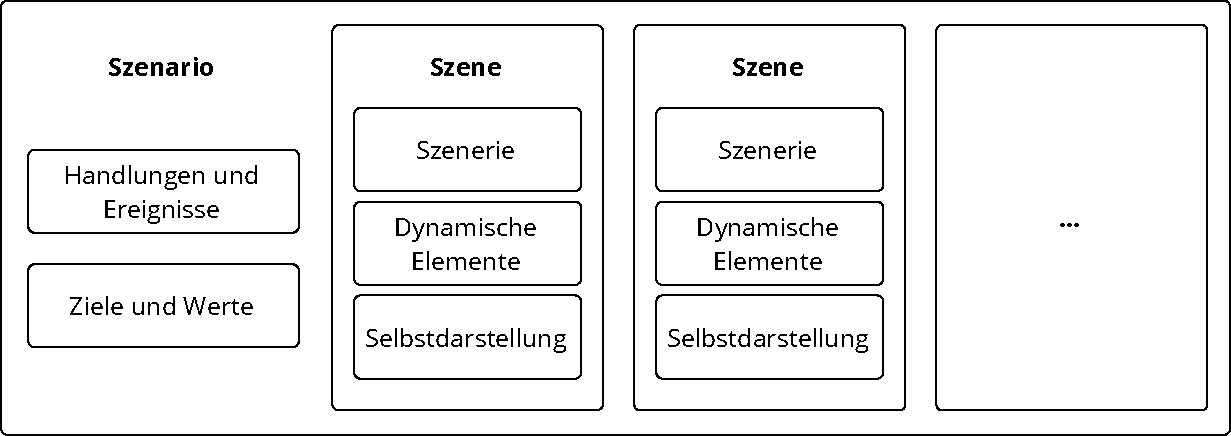
\includegraphics[scale=0.7]{images/relation_sc_sc.pdf}
\caption[Zusammenhang zwischen Szene und Szenario]{Zusammenhang zwischen Szene und Szenario \cite{ulbrich2015defining}}
\label{fig_relation_sc_sc}
\end{figure}

Neben den Begriffen Szene, Situation und Szenario wird oft der Begriff Manöver verwendet. Bach et al. \cite{bach2016model} definieren ein Manöver als einen Zustand innerhalb eines Szenarios. Dabei sind Situationen jeweils Übergangsbedingungen zwischen einzelnen Manövern. So setzt sich beispielsweise das Szenario \textit{Überholen} aus den Manövern \textit{Spurwechsel nach links}, \textit{Beschleunigung}, \textit{Spurwechsel nach rechts} und \textit{Bremsvorgang} zusammen. Zwischen den einzelnen Manövern gibt es Situation wie \textit{langsameres Auto voraus} oder \textit{langsameres Auto links überholt}, die jeweils ein neues Manöver einleiten.

Je nachdem, wie granular Szenarien bzw. wie grob Manöver definiert werden, können Szenarien und Manöver nicht klar voneinander abgegrenzt werden. So kann ein einzelnes Manöver auch bereits ein gesamtes Szenario darstellen. Zum Beispiel kann das Manöver \textit{Spurwechsel} bereits als Szenario definiert werden. Aus diesem Grund wird in dieser Arbeit im Folgenden ausschließlich von Szenarien gesprochen.

Da sich diese Arbeit größtenteils auf die Klassifizierung von Szenarien fokussiert, wird in den folgenden Absätzen eine erweiterte Definition von Szenarien nach Bagschik et al. \cite{bagschik2017szenarien} gegeben. Diese Definition unterteilt den Begriff in drei weitere Abstraktionsebenen: Funktionale, logische und konkrete Szenarien.

Funktionale Szenarien sind auf der semantischen Ebene formuliert. Entitäten und Beziehungen werden widerspruchsfrei in sprachlichen Texten beschrieben. Dabei ist das Vokabular klar definiert und wird eindeutig für alle zu beschreibenden Szenarien verwendet. Je nachdem wie detailliert ein Szenario beschrieben werden soll, muss ein geeignetes Vokabular definiert werden. Funktionale Szenarien können in einzelne oder mehrere logische Szenarien überführt werden.

Logische Szenarien sind detaillierter als funktionale Szenarien, indem  Entitäten und Beziehung in quantitive Parameterbereiche übersetzt werden. Parameterbereiche können dabei mit statistischen Verteilungen (Normalverteilung, Gleichverteilung etc.) modelliert werden. Zusätzlich können Beziehungen zwischen Entitäten mit numerischen Bedingungen (e.g. Fahrzeug A muss auf derselben Spur fahren wie Fahrzeug B) oder Korrelationsfunktionen (e.g. Abstand zwischen Fahrzeug A und Fahrzeug B in Abhängigkeit der Geschwindigkeit) ausgedrückt werden.

Konkrete Szenarien haben den höchsten Detailgrad und Entitäten und Beziehungen werden mit festen Parametern definiert. Logische Szenarien können in einzelne oder mehrere konkrete Szenarien überführt werden.

Ein Beispiel zu jeder Abstraktionsebene (funktional, logisch, konkret) ist in Abbildung \ref{fig_funktional_logisch_konrekt} gegeben.

\begin{figure}[h]
\centering
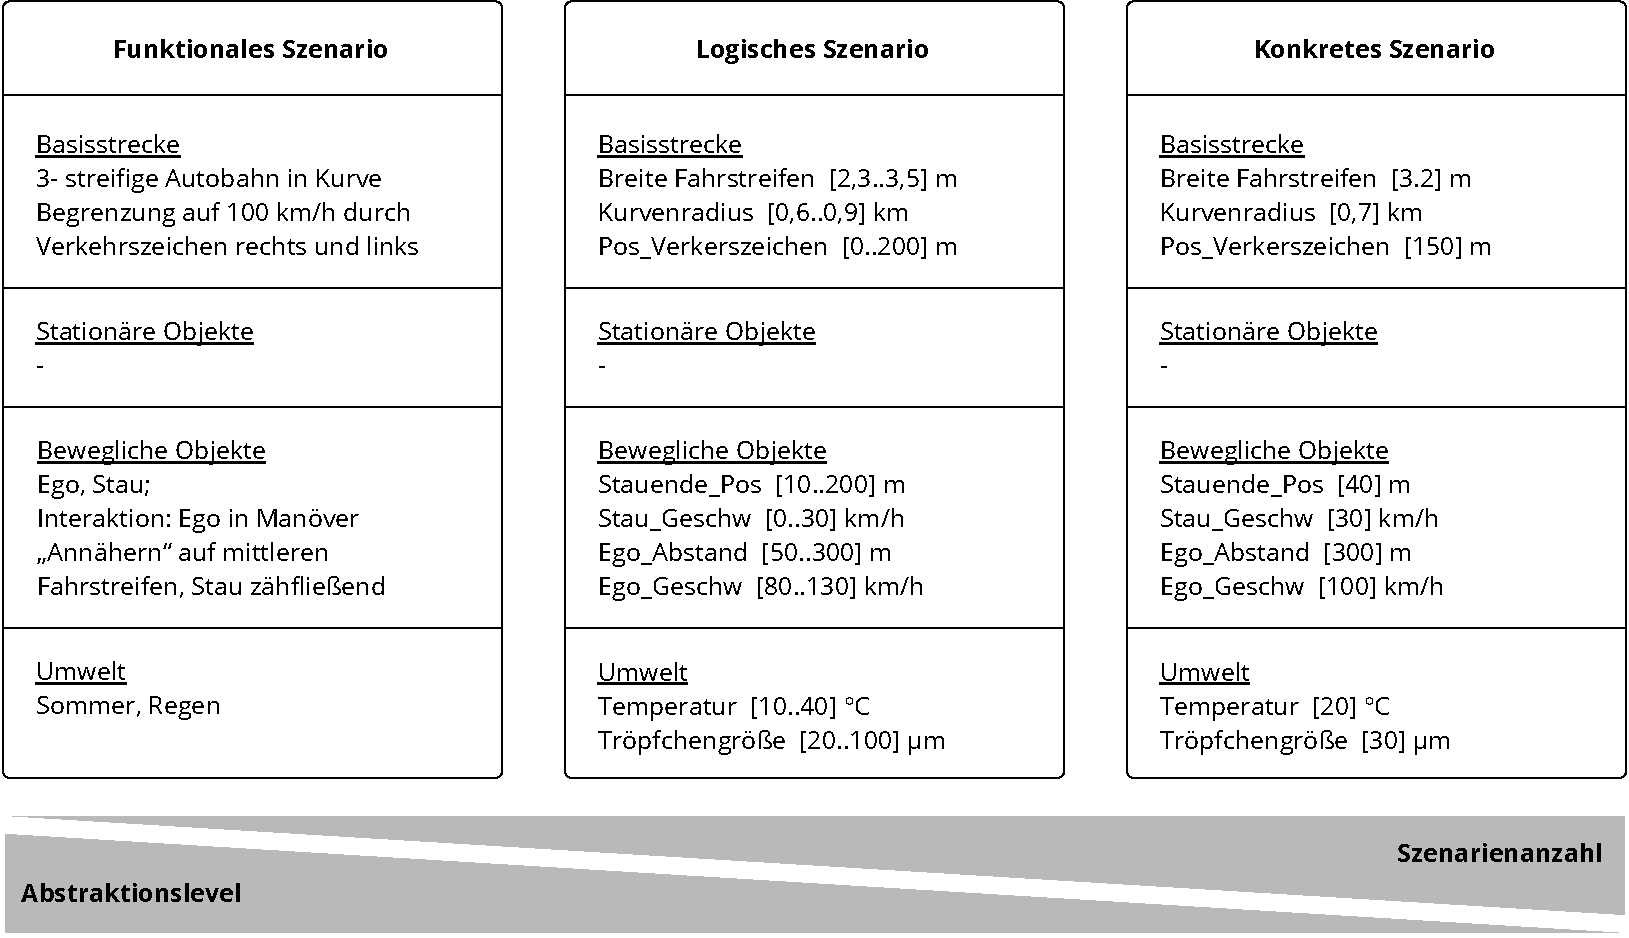
\includegraphics[scale=0.5]{images/funktional_logisch_konrekt.pdf}
\caption[Beispiel für ein funktionales, logisches und konkretes Szenario]{Beispiel für ein funktionales, logisches und konkretes Szenario \cite{bagschik2017szenarien}}
\label{fig_funktional_logisch_konrekt}
\end{figure}


% ===========================
\subsubsection{Bisherige Arbeiten zur Klassifizierung von Fahrszenarien}
% ===========================

Wie in Abschnitt \ref{grundlagen_fahren_entwicklung} beschrieben ist die Klassifizierung von Szenarien ein wichtiges Element für die Erstellung von Testfällen und die Sicherung von \ac{FAS}. In den vergangenen Jahren wurden bereits einige Arbeiten zur Klassifizierung von Szenarien veröffentlicht. In den folgenden Absätzen werden jeweils die Datenbasis, die Klassifizierungsmethode und die jeweiligen Fahrszenarien der bisherigen Arbeiten seit 2014 kurz vorgestellt.

Für die Klassifizierung wurden verschiedene Sensordaten aus dem Fahrzeug verwendet. Die Autoren von fünf Arbeiten haben Beschleunigungs-, Gyroskop-, GPS- und Magnetometer-Daten mithilfe eines Smartphones ein einem Fahrzeug für die Klassifizierung aufgezeichnet \cite{xie2018driving, cervantes2016vehicle, woo2016manoeuvre, camlica2016feature, arroyo2016adaptive}. Die Verwendung von Smartphone-Daten wurde mit der einfachen und kostengünstigen Umsetzung begründet. Vier andere Arbeiten verwendeten Sensordaten wie \textit{Lenkwinkel}, \textit{Fahrzeuggeschwindigkeit}, \textit{laterale Geschwindigkeit}, \textit{Giergeschwindigkeit} und die \textit{Position des Gas- und Bremspedals}, die sie aus dem CAN-Bus des Fahrzeugs auslasen \cite{zheng2017lane, zheng2015non, li2015lane, zheng2014threshold}. Drei weitere Arbeiten basierten ihre Experimente auf Daten aus einem Fahrsimulator \cite{sun2017robust, zheng2016drivers} und realen Testfahrten \cite{gruner2017spatiotemporal}. Die verwendeten Daten waren der \textit{laterale Abstand zwischen Fahrzeug und Fahrbahnmarkierung}, \textit{Spurabfahrtsbetrag}, \textit{Beschleunigung}, \textit{Lenkwinkel}, \textit{Lenkgeschwindigkeit}, \textit{Lenkmoment} und \textit{Ort}, \textit{Ausrichtung}, und \textit{Geschwindigkeit} des Ego-Fahrzeugs und benachbarten Objekten. Dabei wurde nicht weiter spezifiziert, wie die Daten ausgelesen wurden.

Auf Basis der Sensordaten wurden verschiedene Klassifikatoren erstellt. Es wurden die Methoden \ac{SVM} \cite{sun2017robust, cervantes2016vehicle, woo2016manoeuvre, camlica2016feature, zheng2016drivers, zheng2015non}, \ac{RF} \cite{xie2018driving, cervantes2016vehicle, zheng2016drivers}, \ac{kNN} \cite{zheng2017lane, camlica2016feature, zheng2016drivers}, \ac{HMM} \cite{zheng2017lane, li2015lane}, \ac{FRC} \cite{cervantes2016vehicle, arroyo2016adaptive}, Bayesian Inference Model \cite{sun2017robust}, \ac{CNN} \cite{gruner2017spatiotemporal}, Decision Tree \cite{zheng2014threshold} und Naive Bayes \cite{camlica2016feature} verwendet. Da die Methoden für diese Arbeit nicht weiter relevant sind, werden die an dieser Stelle nicht im Detail erläutert, es wird lediglich auf die jeweiligen Quellen verwiesen.

In Tabelle \ref{tab_szenarienerkennung} sind alle dem Autor bekannten Arbeiten seit 2014 zusammengefasst. Neben den verwendeten Methoden zur Klassifizierung sind die jeweils verwendeten Sensordaten und die klassifizierten Szenarien aufgeführt.

\begin{longtable}[c]{p{1,5cm} p{4.5cm} p{2,5cm} p{4.5cm}}
\textbf{Quelle} & \textbf{Sensordaten} & \textbf{Klassifikator} & \textbf{Szenarien} \\
\hline
\endhead

\cite{xie2018driving} & Beschleunigung, Gyroskop und GPS von einem Smartphone das im Fahrzeug platziert ist & \ac{RF} & Abbiegen, links abbiegen, rechts abbiegen, beschleunigen, bremsen, stoppen, Spurwechsel nach links, Spurwechsel nach rechts \\
\hline

\cite{zheng2017lane} & Lenkwinkel und Fahrzeuggeschwindwigkeit aus dem CAN-Bus & \ac{kNN}, \ac{HMM} & Spurwechsel nach links, Spurwechsel nach rechts, Spur halten \\
\hline

\cite{sun2017robust} & Lateraler Abstand zwischen Fahrzeug und Fahrbahnmarkierung von einem Fahrsimulator & \ac{SVM}, Bayesian Inference Model & Spurwechsel nach links, Spurwechsel nach rechts, Spur halten \\
\hline

\cite{gruner2017spatiotemporal} & Ort, Ausrichtung und Geschwindigkeit des Ego-Fahrzeugs und benachbarten Objekten von realen Testfahrten & \ac{CNN} auf Basis von gestapelten Positionsgittern der Objekte & Frei fahren, anderes Fahrzeug voraus, anderes Fahrzeug überholt Ego-Fahrzeug, Querverkehr vor Ego-Fahrzeug \\
\hline

\cite{cervantes2016vehicle} & Beschleunigung von einem Smartphone das im Fahrzeug platziert ist & \ac{RF}, \ac{SVM}, \ac{FRC} & Einparken, geparkt, frei fahren, stoppen \\
\hline

\cite{woo2016manoeuvre} & Beschleunigung, Gyroskop, GPS und Magnetometer von einem Smartphone das im Fahrzeug platziert ist & \ac{SVM} & Stoppen, beschleunigen, bremsen, links abbiegen, rechts abbiegen \\
\hline

\cite{camlica2016feature} & Beschleunigung, Gyroskop und GPS von einem Smartphone das im Fahrzeug platziert ist & \ac{SVM}, \ac{kNN}, Naive-Bayes & Stoppen, beschleunigen, frei fahren, bremsen, Spurwechsel nach links, Spurwechsel nach rechts, links abbiegen, rechts abbiegen, in Kreisverkehr eintreten, aus Kreisverkehr austreten \\
\hline

\cite{zheng2016drivers} & Spurabfahrtsbetrag, Beschleunigung, Lenkwinkel, Lenkgeschwindigkeit und Lenkmoment von einem Fahrsimulator & \ac{SVM}, \ac{kNN}, \ac{RF} & Spurwechsel nach links, Spurwechsel nach rechts, Spur halten \\
\hline

\cite{arroyo2016adaptive} & Beschleunigung, Gyroskop und GPS von einem Smartphone das im Fahrzeug platziert ist & \ac{FRC} & Lenken, beschleunigen, bremsen, Bodenwelle \\
\hline

\cite{zheng2015non} & Fahrzeuggeschwindigkeit und Lenkwinkel aus dem CAN-Bus & \ac{SVM} & links abbiegen, rechts abbiegen, Spurwechsel nach links, Spurwechsel nach rechts, Kurve nach links, Kurve nach rechts, geradeaus fahren, stoppen \\
\hline

\cite{li2015lane} & Fahrzeuggeschwindigkeit, Position des Gas- und Bremspedals, Lenkwinkel, Laterale Beschleunigung und Giergeschwindigkeit aus dem CAN-Bus & \ac{HMM} & Spurwechsel nach links, Spurwechsel nach rechts, Spur halten \\
\hline

\cite{zheng2014threshold} & Fahrzeuggeschwindigkeit, Lenkwinkel, Drehzahl und Position des Gas- und Bremspedals aus dem CAN-Bus & Decision Tree auf Basis von Schwellenwerten & links abbiegen, rechts abbiegen, Spurwechsel nach links, Spurwechsel nach rechts, Kurve nach links, Kurve nach rechts, geradeaus fahren, stoppen \\

\hline
\caption{Bisherige Arbeiten zur Szenarienerkennung}
\label{tab_szenarienerkennung}
\end{longtable}

Die Datenerhebungen in den vergangenen Arbeiten wurde vor dem Hintergrund durchgeführt, vordefinierte Szenarien zu erkennen. Von diesen Szenarien wurden die benötigten Sensordaten abgeleitet und dann mit bestimmten Methoden verschiedene Klassifikatoren erstellt. Bis auf in der Arbeit von Gruner \cite{gruner2017spatiotemporal} werden für die Klassifizierung von Fahrszenarien bisher keine \acp{DNN} verwendet. Ebenfalls verwendet Gruner in seiner Arbeit keine Kamerabildern, sondern gespapelte Matritzen, auf denen jeweils die Positionen aller Verkehrsteilnehmer markiert sind. Nach Gruner \cite{gruner2017spatiotemporal} wird sich die zukünftige Forschung mit tieferen Netzstrukturen wie Recurrent Neural Networks (\acp{RNN}) beschäftigen, um zeitabhängige Szenarien noch besser zu verstehen.

Mit den bisherigen Ansätzen können bekannte Szenarien sehr zuverlässig erkannt werden. Bisher unbekannte Szenarien werden allerdings nur sehr bedingt erkannt, weil die Datengrundlage auf Basis der bekannten Szenarien optimiert ist. Das bedeutet, dass Daten, die für die Erkennung von bisher unbekannten Szenarien möglicherweise relevant sind, nicht erfasst und daher nicht für die Erstellung des Klassifikators verwendet werden.

Im Gegensatz zu den bisherigen Arbeiten, soll in dieser Arbeit die Verwendung von Kameradaten für die Klassifizierung von Szenarien untersucht werden. Die Idee ist, dass Videodaten den gleichen Informationsgehalt besitzen wie das Sichtfeld eines realen Fahrers. Ein Fahrer kann auf Basis seines Sichtfeldes alle Szenarien erkennen und auf der Basis die Umgebung und alle Fahrfunktionen überwachen. Da in Zukunft das System diese Aufgabe übernehmen wird, soll in dieser Arbeit ein Klassifikator mit genau diesem Sichtfeld, mit Videodaten, trainiert werden. Damit sollen auch bisher unbekannte Einflüsse, die auf den Bildern zu sehen sind, für die Klassifizierung berücksichtigt werden. In einem weiteren Schritt kann ein Klassifikator, der auf diese Weise mit allen bisher bekannten Szenarien trainiert wurde, bekannte Szenarien erkennen und bisher unbekannte Szenarien identifizieren. Der Ansatz wird im Detail in Kapitel \ref{konzept} vorgestellt.

% ===========================
\section{Künstliche Neuronale Netze}
\label{grundlagen_nn}
% ===========================

In diesem Kapitel werden künstliche Neuronale Netze (\acp{KNN}) mit mit einem Schwerpunkt auf Bilderkennung mit Convolutional Neural Networks (\acp{CNN}) und Sequenzerkennung mit \acp{LSTM} eingeführt. Im folgenden Abschnitt \ref{grundlagen_nn_ml} werden \acp{KNN} in den Gesamtkontext von maschinellem Lernen gestellt. Im Anschluss werden in Abschnitt \ref{grundlagen_nn_entwicklung} die Grundlagen zu \acp{KNN} erläutert. Dann werden komplexe Architekturen von \acp{KNN} zur Bilderkennung in Abschnitt \ref{grundlagen_nn_cnn} und zur Sequenzerkennung in Abschnitt \ref{grundlagen_nn_rnn} erklärt. In Abschnitt \ref{grundlagen_nn_synthetisch} wird auf das Training mit synthetischen Daten eingegangen und im letzten Abschnitt \ref{grundlagen_nn_video} wird die aktuelle Forschung zu Videoklassifizierung vorgestellt.

% ===========================
\subsection{Einordnung im maschinellen Lernen}
\label{grundlagen_nn_ml}
% ===========================

Maschinelles Lernen wird oft als ein Teil des Bereichs künstliche Intelligenz beschrieben. Dabei wird maschinelles Lernen nach Mitchell \cite{mitchell1997machine} wie folgt definiert:

\begin{quote}
\textit{\glqq Ein Computerprogramm lernt aus der Erfahrung E in Bezug auf eine Klasse von Aufgaben T und dem Leistungsmaß P, wenn seine Leistung, gemessen mit P, bei Aufgaben aus T sich mit Erfahrung E verbessert.\grqq}
\end{quote}

Da maschinelles Lernen sehr viele Bereiche umfasst, wird hier nur auf die relevanten Teile für diese Arbeit eingegangen und auf \cite{mitchell1997machine} verwiesen. Maschinelles Lernen kann in drei verschiedenen Kategorien eingeteilt werden. Diese werden in den folgenden Absätzen beschrieben.

Überwachtes Lernen (engl. supervised learning) beschreibt einen Lernprozess, in dem die Trainingsdaten sowohl Inputvektoren als auch die zugehörigen Zielvektoren enthalten \cite{bishop2006pattern}. Ein Beispiel dafür ist ein Klassifizierungsproblem von Buchstaben, bei dem sowohl die Bilder der einzelnen Buchstaben, als auch deren zugehörige Klasse (abgebildeter Buchstabe) einem Trainingsalgorithmus übergeben werden. Neben Klassifizierungsproblemen fallen auch Regressionsprobleme in diese Kategorie.

Beim unüberwachten Lernen (engl. unsupervised learning) enthalten die Trainingsdaten ausschließlich die Inputvektoren, ohne die dazugehörigen Zielvektoren. Das Ziel dabei ist es, Muster in den gegebenen Daten zu erkennen, um beispielsweise Cluster zu bilden \cite{bishop2006pattern}. Das Clustering von Kundengruppen, die bisher unbekannt waren, fällt in diese Kategorie des maschinellen Lernens.

Das verstärkende Lernen (engl. reinforcement learning) ist eine Methodik in welcher der Trainingsalgorithmus mit Situationen konfrontiert wird und jeweils aus einer Reihe von gegebenen Handlungen wählen kann. Das Ziel dabei ist es das Endergebnis, das auf der Wahl aller Handlungen basiert, zu maximieren \cite{sutton1998introduction}. Ein Beispiel hierfür ist selbstständige Erlernen des Brettspiels Schach.


% ===========================
\subsubsection{Klassifizierung}
% ===========================

In dieser Arbeit wird ein Konzept für die Klassifizierung von Fahrszenarien - damit in der Kategorie überwachtes Lernen - entwickelt und umgesetzt. Das Ziel von Klassifizierungsalgorithmen ist es, gegebene Objekte auf Basis ihrer Eigenschaften einer Klasse zuzuordnen. Dabei sollen die Objekte innerhalb einer Klasse eine möglichst geringe Varianz und zwischen verschiedenen Klassen eine möglichst hohe Varianz besitzen. Klassifizierungsalgorithmen arbeiten dafür mit Trainingsdaten, die aus Inputvektoren und Zielvektoren bestehen. Ein Inputvektor enthält alle Eigenschaften und der Zielvektor die jeweilige Klasse des Objekts. In Abbildung \ref{fig_klassifizierung} ist beispielhaft ein Datensatz mit zwei Klassen dargestellt. Die Objekte im Datensatz haben jeweils die Eigenschaften $x_1$ und $x_2$.

\begin{figure}[h]
\centering
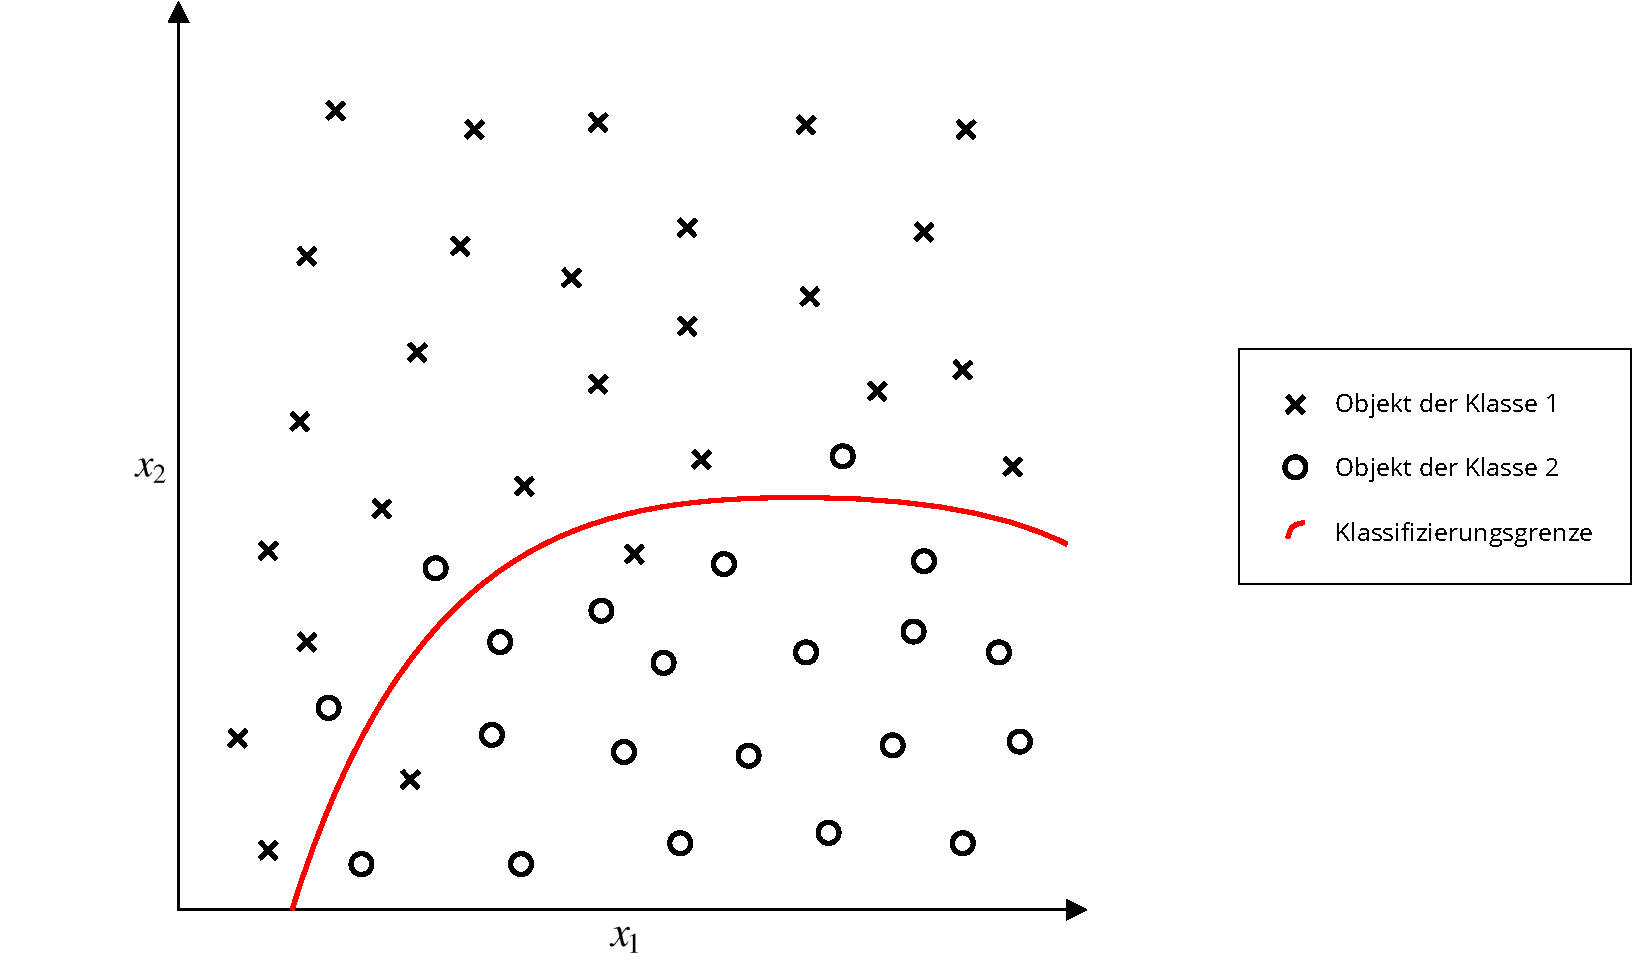
\includegraphics[scale=0.5]{images/klassifizierung.pdf}
\caption{Beispiel einer Klassifizierung mit zwei Klassen}
\label{fig_klassifizierung}
\end{figure}

In den folgenden Abschnitten werden schrittweise \acp{CNN} und \acp{LSTM} eingeführt, mit denen in dieser Arbeit ein Klassifikator für die Erkennung von Fahrszenarien entwickelt und trainiert wird.


% ===========================
\subsection{Entwicklung von künstlichen neuronalen Netzen}
\label{grundlagen_nn_entwicklung}
% ===========================

\acp{KNN} wurden ursprünglich als ein Modell der Informationsverarbeitung von biologischen Gehirnen entwickelt \cite{mcculloch1943logical}. Dabei ist die kleinste Einheit in einem \ac{KNN} ein einzelnes Neuron. Rosenblatt \cite{rosenblatt1958perceptron} entwickelte ein Modell eines Neurons als binären Klassifikator. Dieses sogenannte Perzeptron setzt sich aus einem Eingangsvektor $x_1, ..., x_n$, einem Vektor mit Gewichten $w_1, ..., w_n$, einer Summenfunktion $\sum$, einer Aktivierungsfunktion $\varphi$ mit einem Schwellenwert $\theta$ und einem Aktivierungswert $o(\vec{x})$ zusammen. Abbildung \ref{fig_perceptron} zeigt das Modell eines Perzeptrons.

\begin{figure}[h]
\centering
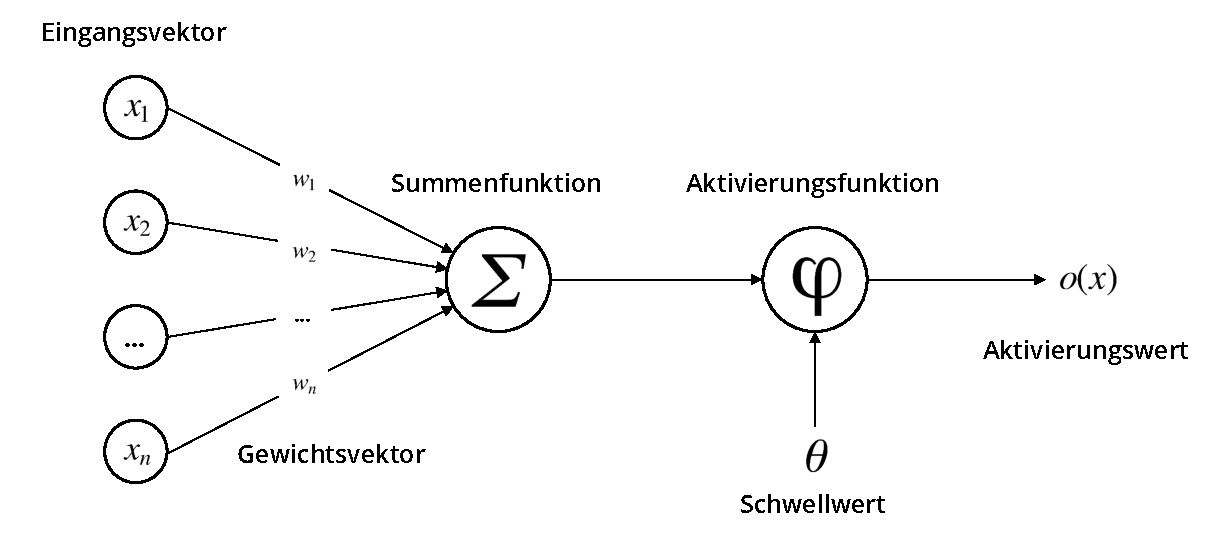
\includegraphics[scale=0.7]{images/perceptron.pdf}
\caption[Modell eines Perzeptrons]{Modell eines Perzeptrons \cite{rosenblatt1958perceptron}}
\label{fig_perceptron}
\end{figure}

Um den Aktivierungswert $o(\vec{x})$ zu berechnen wird zunächst die gewichtete Summe mit dem Eingangsvektor $\vec{x}$ und den Gewichten $\vec{w}$ gebildet. Dann wird mit der Aktivierungsfunktion $\varphi$ eine Klasse bestimmt. Beim ursprünglichen Perzeptron handelt es sich dabei um eine Schwellenwertfunktion, die die zwei Werte $-1$ und $1$ annehmen kann. Damit ist das Perzeptron ein binärer Klassifikator und kann die logischen Operationen \textit{AND}, \textit{OR} und \textit{NOT} ausführen. Die logische Operation \textit{XOR} kann mit mit einem einzelnen Perzeptron nicht abgebildet werden \cite{minski1969perceptrons}.

\begin{equation}
\varphi(\vec{x}, \vec{w}) = \begin{cases} 1 \qquad \text{wenn} \quad \vec{x}*\vec{w} \geq \theta \\ 0 \qquad \text{sonst} \end{cases}
\end{equation}

Die Klassifizierung eines Objekts aus der Klasse $t$ mit den Eigenschaften $\vec{x}$ ist richtig, wenn das Ergebnis $o$ der Aktivierungsfunktion $\varphi(\vec{x},\vec{w})$ der tatsächlichen Klasse des Objekts $t$ entspricht. Wenn die Klasse nicht richtig erkannt wurde $o(\vec{x}) \neq t$, werden die Gewichte $\vec{w}$ entsprechend der Perzeptron-Lernregel angepasst. Diese Lernregel ist ein wichtiger Vorteil von Rosenblatts Perzeptron \cite{rosenblatt1958perceptron} gegenüber des Neurons von McCulloch und Pitts \cite{mcculloch1943logical}, weil die Gewichte erlernt werden können.

Vor dem Training werden die Gewichte $\vec{w}$ zufällig initialisiert. In jedem Trainingsschritt wird überprüft ob die berechnete Klasse $o(\vec{x})$ der tatsächlichen Klasse $t$ entspricht. Wenn $o(\vec{x}) = t$ werden die Gewichte nicht verändert und der nächste Trainingsschritt wird ausgeführt. Wenn $o(\vec{x}) \neq t$ werden die Gewichte nach der Perzeptron-Lernregel aktualisiert:

\begin{equation}
w^{neu}_i = w^{alt}_i + \Delta w_i
\end{equation}
\begin{equation}
\Delta w_i = \eta*(t-o)*x_i
\end{equation}

Die Lernrate $\eta$ kann angepasst werden und bestimmt wie stark die Gewichte in jedem Trainingsschritt verändert werden. Üblicherweise werden Lernraten zwischen $1e-2$ und $1e-4$ gewählt.

Neben der Schwellenwertfunktion werden für die Aktivierung von einzelnen Neuronen verschiedene Aktivierungsfunktionen verwendet. Die am meisten verwendeten Funktionen hierfür sind die \ac{tanh}-Funktion

\begin{equation}
\varphi(x) = \tanh(x) = \frac{e^{2x}-1}{e^{2x}+1} \text{,}
\end{equation}

\noindent die Sigmoid- oder S-Funktion

\begin{equation}
\varphi(x) = \frac{1}{1+e^{-x}}
\end{equation}

\noindent und die \ac{ReLU}-Funktion 

\begin{equation}
\varphi(x) = \max{(0, x)}.
\end{equation}

\noindent Diese Funktionen sind, zusammen mit der zuvor vorgestellten Schwellenwertfunktion, in Abbildung \ref{fig_aktivierungsfunktionen} dargestellt.

\begin{figure}[h]
\centering
\begin{tabular}{cc}
\subfloat[Sigmoid]{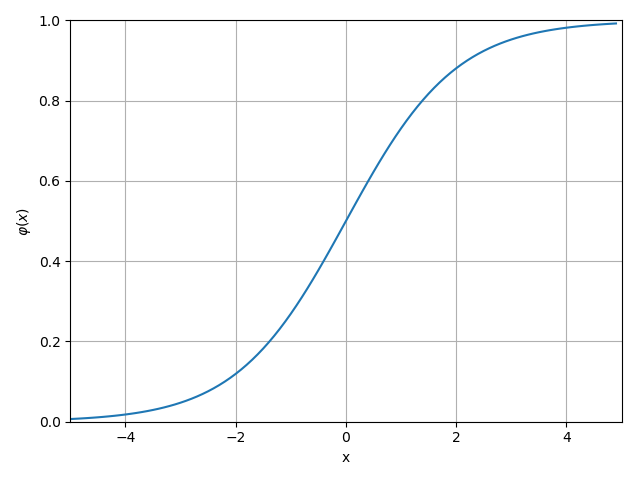
\includegraphics[scale=0.4]{images/act_sigmoid.png}} &
\subfloat[\ac{tanh}]{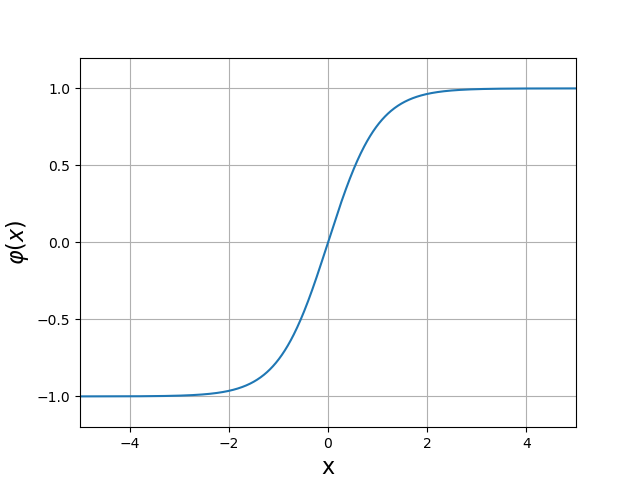
\includegraphics[scale=0.4]{images/act_tanh.png}} \\
\subfloat[\ac{ReLU}]{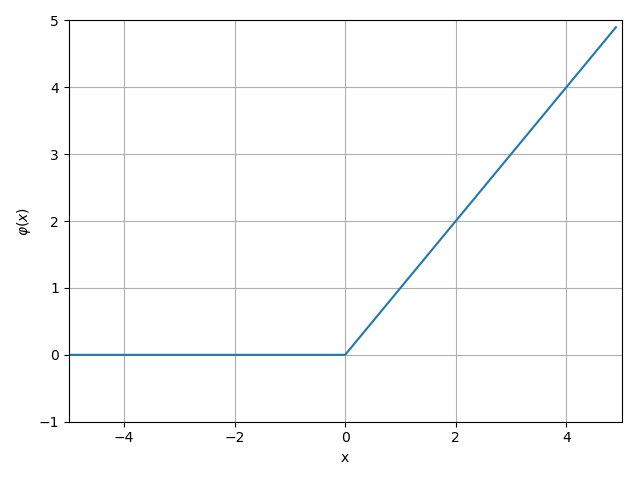
\includegraphics[scale=0.4]{images/act_relu.png}} &
\subfloat[Schwellenwertfunktion]{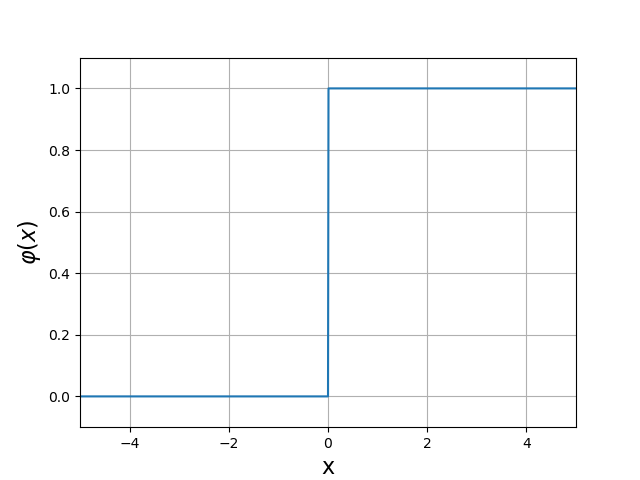
\includegraphics[scale=0.4]{images/act_step_fc.png}}
\end{tabular}
\caption{Aktivierungsfunktionen für Neuronen}
\label{fig_aktivierungsfunktionen}
\end{figure}

Mit diesen Aktivierungsfunktionen und der Verwendung mehrerer Perzeptronen werden mehrschichtige \acp{KNN}, oder auch mehrlagiges Perzeptron (engl. multilayer perceptron), modelliert. Dadurch können diese auf unterschiedliche Probleme angewendet werden und überwinden die Schwächen eines einzelnen Perzeptrons (ausschließlich binäre Klassifizierung, keine \textit{XOR}-Operation). Ein mehrschichtiges \ac{KNN} besteht aus mindestens zwei Schichten, einer Ergebnis-Schicht und mindestens einer verborgenen Schicht. Der Eingangsvektor $\vec{x}$ wird nicht als eine Schicht gezählt. Jede Schicht besteht aus $1, ..., n$ Neuronen (Perzeptronen), die im Modell als Knoten modelliert sind. Die Neuronen einer Schicht bestehen jeweils aus einer gewichteten Summe und einer Aktivierungsfunktion und sind jeweils mit dem Eingangsvektor, dem Ergebnisvektor oder den Neuronen der vorherigen und nachfolgenden Schichten verbunden. Diese Verbindungen werden als Kanten modelliert und repräsentieren die Gewichte mit denen die Neuronen verknüpft sind. Abbildung \ref{fig_knn} zeigt das Schema eines dreischichtigen \ac{KNN}.

\begin{figure}[h]
\centering
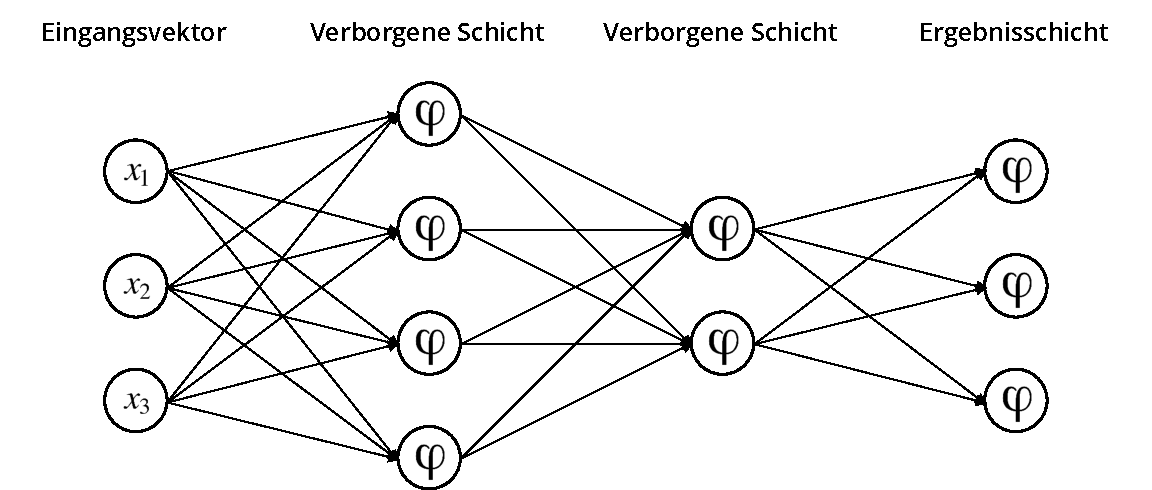
\includegraphics[scale=0.7]{images/knn.pdf}
\caption{Mehrlagiges Perzeptron mit zwei versteckten Schichten und einer Ausgangsschicht}
\label{fig_knn}
\end{figure}

Das Training eines mehrschichtigen \ac{KNN} funktioniert analog zu dem Training eines einzelnen Perzeptrons. In jedem Trainingsschritt wird ein Ergebnis $o(\vec{x})$ berechnet und mit dem richtigen Ergebnis $t$ verglichen. Mit dem Eingangsvektor $\vec{x}$ werden die Aktivierungswerte $y_j$ des Vektors  $\vec{y}$ der ersten verborgenen Schicht wie folgt berechnet:

\begin{equation}
y_j = \varphi(\sum_i{w_{ij}*x_i})
\end{equation}

Dabei ist $w_{ij}$ die Gewichtung der Kante zwischen dem Eingangswert $x_i$ und dem verborgenem Neuron $j$. Alle weiteren verborgenen Schichten sowie der Ergebnisvektor werden auf die gleiche Weise, mit den Aktivierungswerten der vorherigen Schicht als Eingangsvektor, berechnet. Für binäre Klassifizierungsprobleme kann beispielsweise die Sigmoid-Funktion als Aktivierungsfunktion für die Ergebnisschicht gewählt werden. Dann ist das Ergebnis $o$ eine Zahl zwischen $0$ und $1$ und beschreibt die Wahrscheinlichkeit, dass der Eingangsvektor $\vec{x}$ zur Klasse $c_1$ gehört. Dementsprechend beschreibt $1-o$ die Wahrscheinlichkeit der Klasse $c_2$. Bei Klassifizierungsproblemen mit mehreren Klassen wird häufig die Softmax-Funktion als Aktivierungsfunktion $\varphi$ gewählt, um die Wahrscheinlichkeiten der einzelnen Klassen $c_k$ zu bestimmen \cite{bridle1990probabilistic}:

\begin{equation}
o_k = p(c_k|x) = \frac{e^{x^\top w}}{\sum_{j=1}^Ce^{x_j^\top w}}
\end{equation}

Dabei beschreibt $x$ den Vektor mit Aktivierungswerten aus der vorherigen Schicht, $w$ den Gewichtsvektor und $C$ die Anzahl der Klassen $c_k$. Auf diese Weise können die Wahrscheinlichkeiten $p(c_k|x)$ für jede Klasse $c_k$, gegeben den Aktivierungswerten $x$, berechnet werden.

Für das Erlernen von Gewichten in mehrschichtigen \acp{KNN} wird die Fehlerrückführung (engl. error backpropagation) verwendet. Die Idee bei diesem Verfahren ist es, eine Fehlerfunktion, welche die Abweichung zwischen der berechneten und der tatsächlichen Klasse beschreibt, zu definieren und anschließend zu minimieren \cite{bishop2006pattern}. Dafür wird häufig die mittlere quadratische Abweichung als Fehlerfunktion verwendet:

\begin{equation}
E = \frac{1}{n}\sum_{j=1}^n(t_j-o_j)^2
\end{equation}

Dabei beschreiben $t_j$ die tatsächliche Klasse, $o_j$ die errechnete Klasse und $n$ die Anzahl der Klassen. Auf Basis dieser Fehlerfunktion läuft die Fehlerrückführung iterativ in den folgenden Schritten ab \cite{bishop2006pattern}:

\begin{enumerate}
\item Auf Basis eines Eingangsvektors $\vec{x}$ werden die Aktivierungswerte $\vec{y_j}$ aller versteckten Schichten $j$ und der Ergebnisvektor $\vec{o}$ berechnet.
\item Der errechnete Ergebniswert $o_j$ wird mit dem erwarteten Ergebnis $t_j$ verglichen und die Differenz wird berechnet. Diese Different wird als Fehler bezeichnet.
\item Auf Basis dieser Differenz werden die Gewichte zwischen allen Neuronen geändert, mit dem Ziel diese Differenz bei der nächsten Iteration zu verringern. Die Änderung wird wie folgt berechnet:
\begin{equation}
w^{neu}_{ij} = w^{alt}_{ij} + \Delta w_{ij}
\end{equation}
mit
\begin{equation}
\Delta w_{ij} = -\eta \frac{\partial E}{\partial w_{ij}}
\end{equation}
Dabei beschreibt $w_{ij}$ das Gewicht zwischen Neuron $i$ und Neuron $j$, $\eta$ eine feste Lernrate die beeinflusst, wie stark Gewichte geändert werden und $E$ die oben definierte Fehlerfunktion.
\end{enumerate}

Mit diesem Algorithmus werden die Gewichte von mehrschichtigen \acp{KNN} bei jedem Trainingsschritt angepasst. Eine Herausforderung beim Trainieren von \acp{KNN} ist es, mit bisher unbekannten Daten gute Ergebnisse zu erzielen \cite{srivastava2014dropout}. Das bedeutet, dass im Laufe des Trainings die Gewichte so angepasst werden müssen, dass das Modell nach dem Training nicht nur mit den Trainingsdaten gute Ergebnisse erzielen kann, sondern auch auf Daten, die es zuvor nicht verarbeitet hat. Diese Fähigkeit eines Modells wird Generalisierbarkeit genannt. Wenn ein Modell hingegen nur mit den Trainingsdaten gute Ergebnisse erzielt, spricht man von Überanpassung (engl. overfitting). Im Gegensatz dazu spricht man von Unteranpassung (engl. underfitting), wenn ein Modell schon mit den Trainingsdaten sehr schlechte Ergebnisse erzielt. In Abbildung \ref{fig_overfitting} ist beispielhaft eine Unter- und Überanpassung eines binären Klassifikators dargestellt.

\begin{figure}[h]
\centering
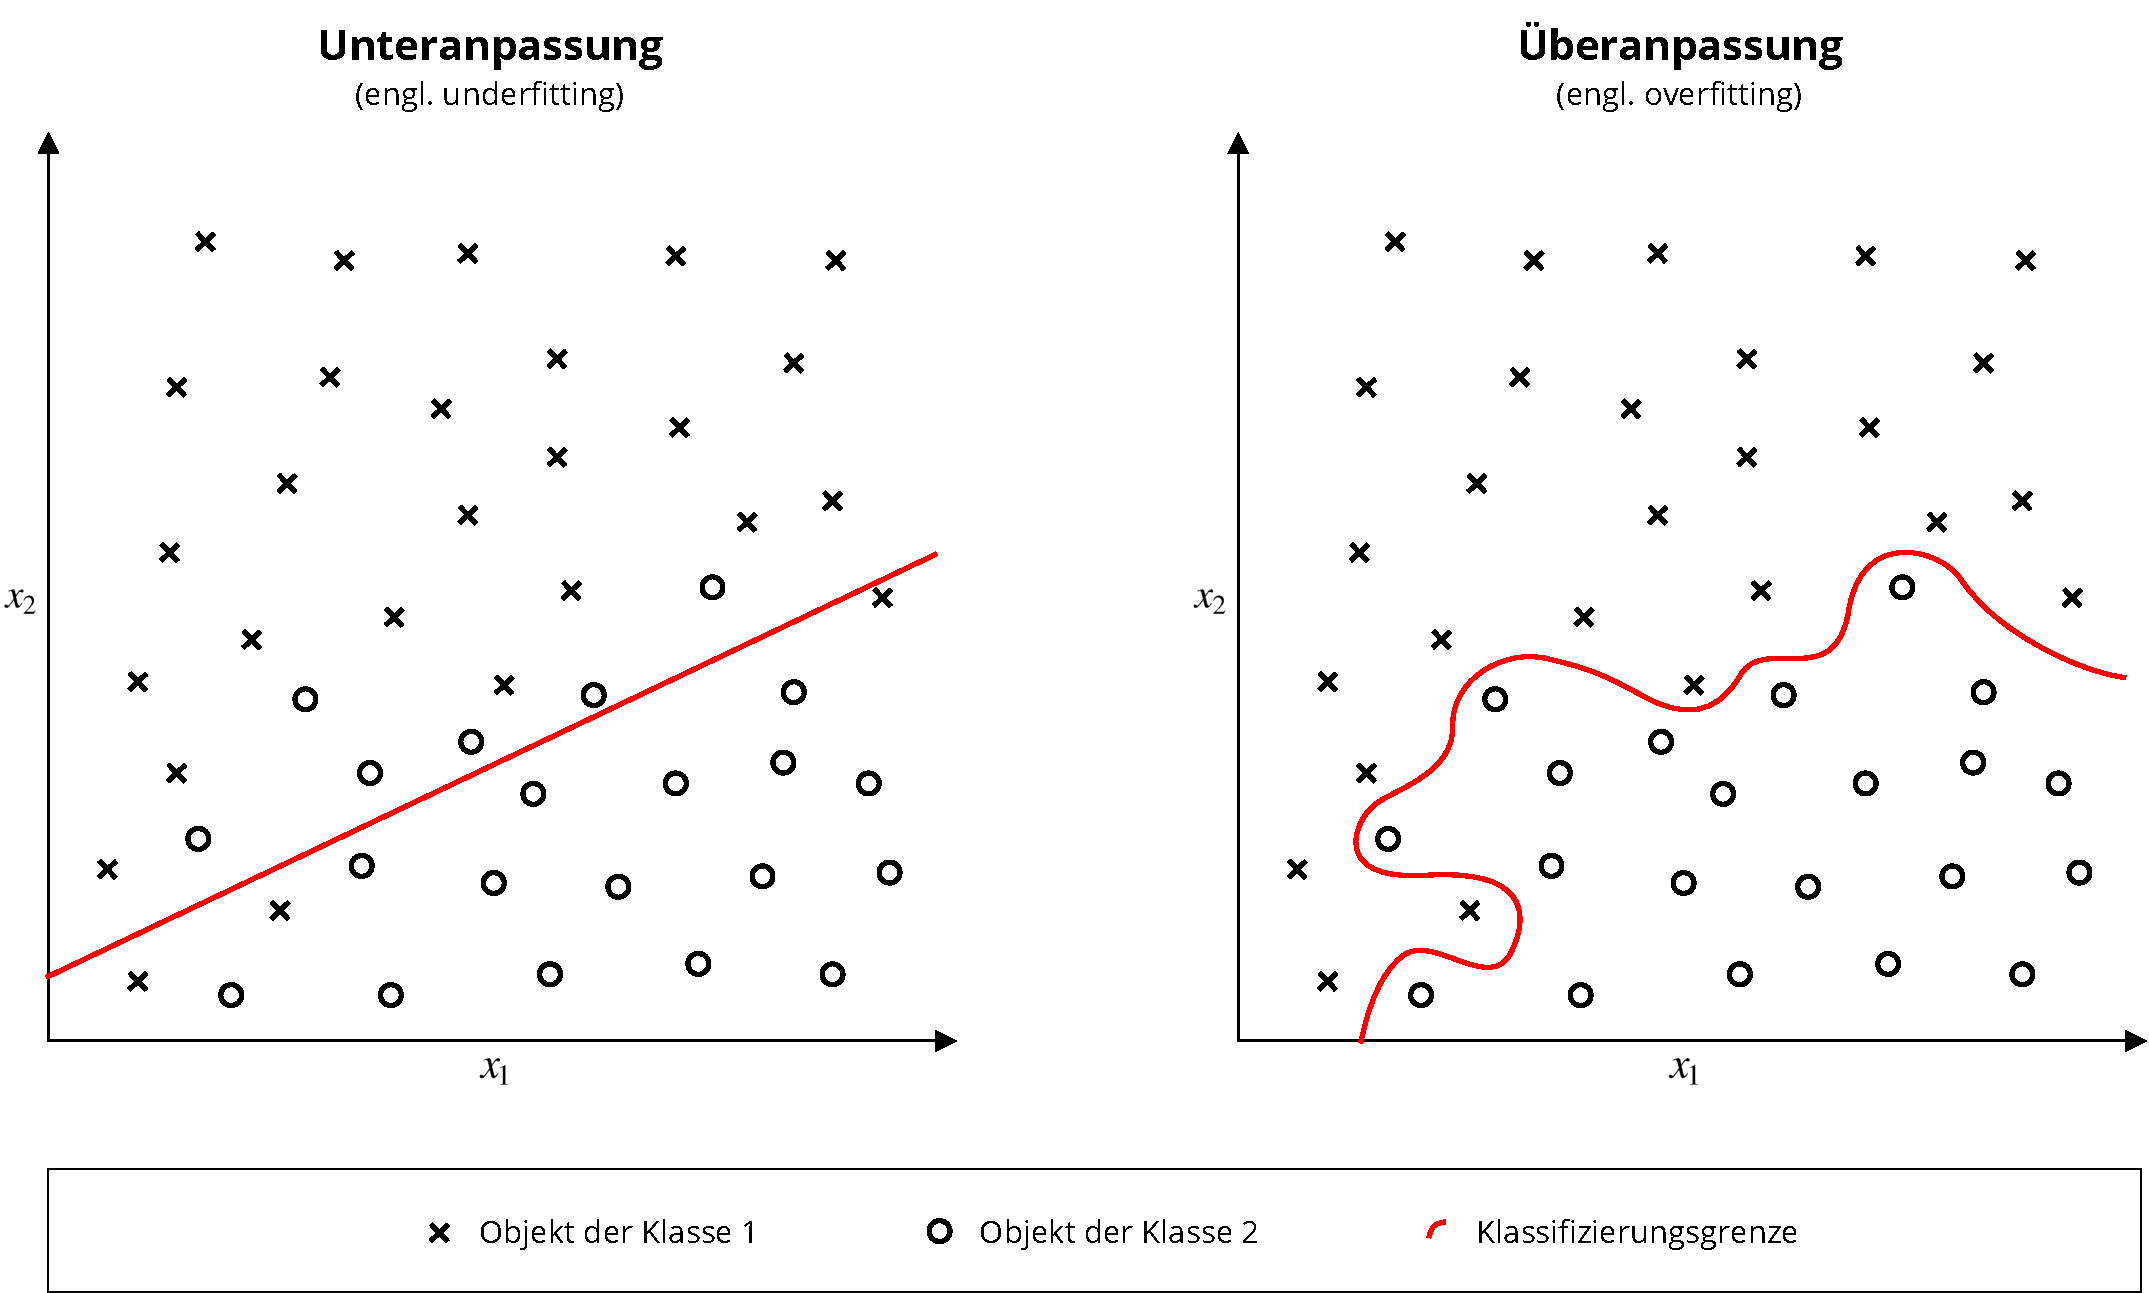
\includegraphics[scale=0.4]{images/overfitting.pdf}
\caption{Beispiel einer Unter- und Überanpassung eines Klassifikators}
\label{fig_overfitting}
\end{figure}

Heute werden in Anwendungen häufig tiefe neuronale Netze (engl. deep neural networks) verwendet. Von einem tiefen neuronalen Netz spricht man, wenn es viele versteckte Schichten besitzt. Damit können Merkmale auf verschiedenen Abstraktionsebenen erkannt werden \cite{lecun2015deep}. In den folgenden Absätzen \ref{grundlagen_nn_cnn} und \ref{grundlagen_nn_rnn} werden zwei verschiedene Architekturen von tiefen neuronalen Netzen vorgestellt, die in Kapitel \ref{umsetzung} für das Klassifizierungsproblem dieser Arbeit angewendet werden.


% ===========================
\subsection{Convolutional Neural Networks}
\label{grundlagen_nn_cnn}
% ===========================

Ein \acf{CNN} ist eine Architektur eines \acp{KNN} und gilt heute als Stand der Technik für Probleme in der Bilderkennung \cite{krizhevsky2012imagenet}. Die Architektur eines \acp{CNN} besteht grundsätzlich aus einer oder mehreren Convolution- und Pooling-Schichten \cite{lecun2010convolutional}. Diese Abfolge kann sich beliebig oft wiederholen und wird am Ende mit einer oder mehreren Fully-Connected-Schicht für die Klassifizierung ergänzt. In den folgenden Absätzen werden die Funktionsweisen der Convolution- und der Pooling-Schicht erklärt. Eine Fully-Connected-Schicht entspricht einer Schicht im mehrlagigen Perzeptron wie sie im vorherigen Abschnitt \ref{grundlagen_nn_entwicklung} beschrieben wurde. In Abbildung \ref{fig_cnn} ist ein gesamtes \ac{CNN} dargestellt.

Die Convolution-Schicht besteht aus einer Convolution-Operation gefolgt von einer Aktivierungsfunktion. Die Grundidee dieser Schicht ist die Extraktion von Merkmalen aus einem Bild oder anderen Inputdaten. Dabei werden in den ersten Schichten Merkmale auf einer niedrigen Ebene (engl. low-level features) und in späteren Schichten zunehmend abstraktere Merkmale (engl. high-level features) extrahiert. Bei der Convolution-Operation (oder auch Faltung) wird ein ausgewählter Filter mit einer festgelegten Schrittgröße (engl. stride) über das Bild bewegt und bei jedem Schritt der entsprechende Ausgabewert berechnet \cite{lecun1998cnn}. Diese Operation ist in Abbildung \ref{fig_conv_operation} dargestellt.

\begin{figure}[h]
\centering
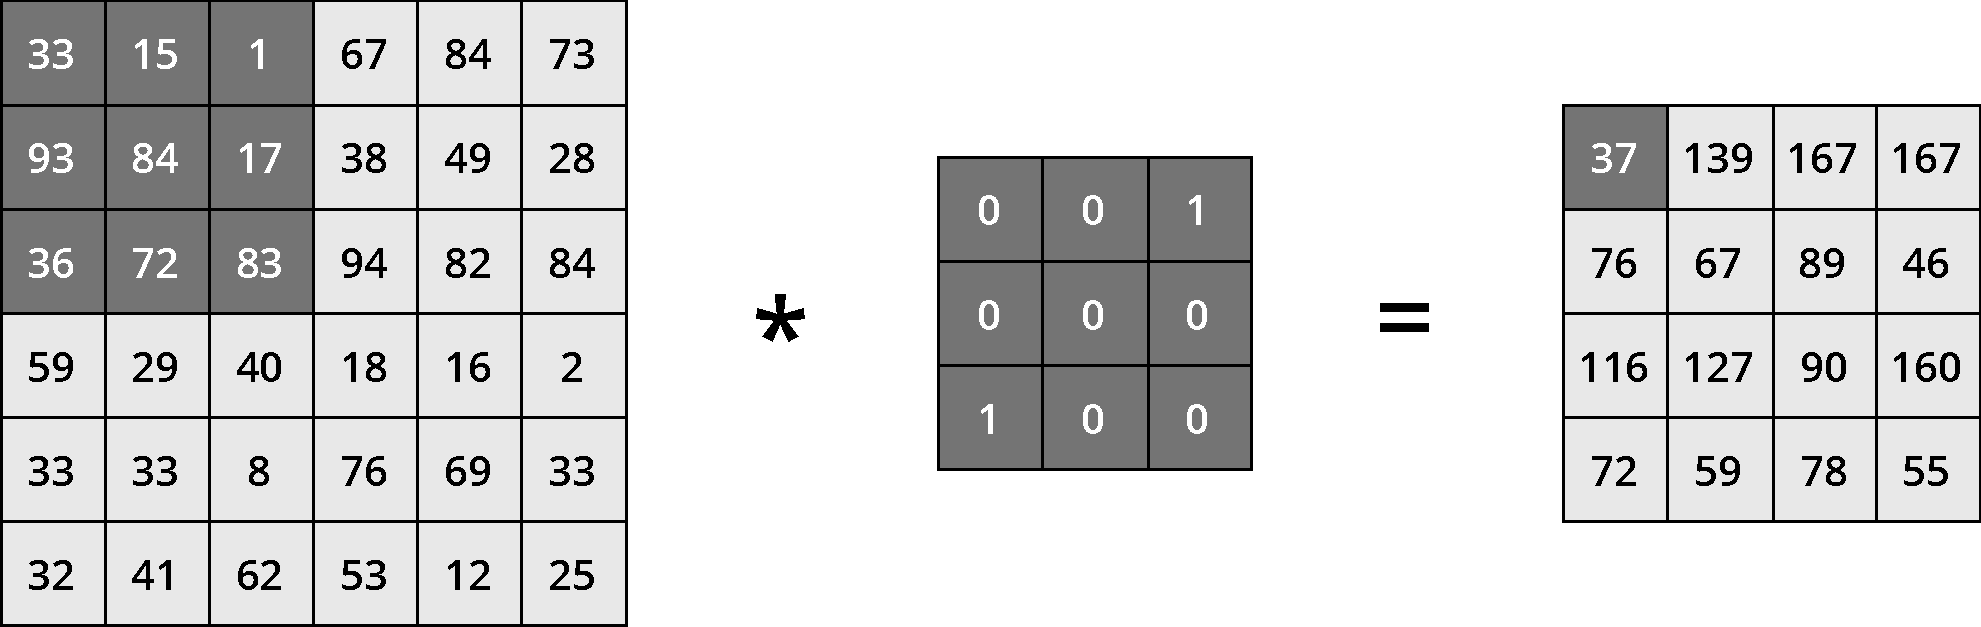
\includegraphics[scale=0.4]{images/conv_operation.pdf}
\caption{Beispiel einer Convolution-Operation}
\label{fig_conv_operation}
\end{figure}

In diesem Beispiel handelt es sich um ein Bild mit den Dimensionen 6x6x1 Pixel, also einem zweidimensionalen Bild mit einem Farbkanal. Der Filter hat die Dimensionen 3x3x1. In dem Beispiel ist die aktuell dargestellte Rechnung wie folgt:

\begin{equation*}
0*33+0*15+1*1+0*93+0*84+0*17+1*36+0*72+0*83=37
\end{equation*}

Nach dieser Berechnung bewegt sich der Filter einen Schritt weiter nach rechts und der nächste Wert wird berechnet. Am rechten Rand des Bildes angekommen, wird der Filter eine Schrittlänge weiter nach unten gesetzt und wieder an den linken Rand gesetzt. Dies wiederholt sich bis der Filter am rechten unteren Rand des Bildes angekommen ist. Bei einem dreidimensionalen Bild, mit den drei Farbkanälen als dritte Dimension, hat der Filter ebenfalls drei Dimensionen. Die Berechnung wird analog durchgeführt. Bei dieser Operation kann die Größe des Filters und die Schrittgrüße variiert werden. Es können auch verschiedenen Filter verwendet werden, um unterschiedliche Merkmale zu extrahieren. Außerdem können sogenannte Padding-Methoden eingesetzt werden um den Rand der Bilder künstlich zu erweitern. Beim sogenannten Zero-Padding wird beispielsweise ein beliebig breiter Rand mit den Werten 0 um das Bild gelegt. Somit kann sich ein Filter auch über die existierenden Ränder hinweg bewegen und Muster an den Rändern besser erkennen. Das Ergebnis einer Convolution Schicht ist eine sogenannte Feature Map, also eine Schicht, die aus extrahierten Merkmalen besteht \cite{lecun1997convolutional}.

Das Ziel der Pooling-Schicht ist es, die Größe der Feature Map zu reduzieren und dabei die wichtigsten Merkmale beizubehalten \cite{scherer2010evaluation}. Wie bei der Convolution-Operation, gibt es auch beim Pooling verschiedene Operationen (z.B. Average-Pooling). In Abbildung \ref{fig_pool_operation} ist die oft verwendete Max-Pooling-Operation dargestellt. Dabei werden Fenster mit einer festgelegten Breite und Höhe über das Bild bewegt und jeweils nur der maximale Wert innerhalb eines Fensters übernommen.

\begin{figure}[h]
\centering
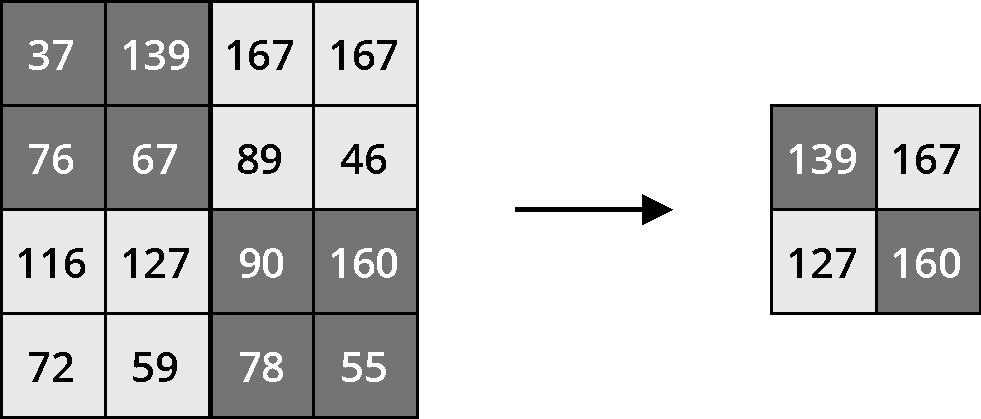
\includegraphics[scale=0.4]{images/pool_operation.pdf}
\caption{Beispiel einer Max-Pooling-Operation}
\label{fig_pool_operation}
\end{figure}

Mit Convolution-, Pooling- und Fully-Connected-Schichten kann die Architektur eines \acp{CNN} zusammengesetzt werden. In Abbildung \ref{fig_cnn} ist beispielhaft die Architektur eines \ac{CNN} abgebildet.


\begin{figure}[h]
\centering
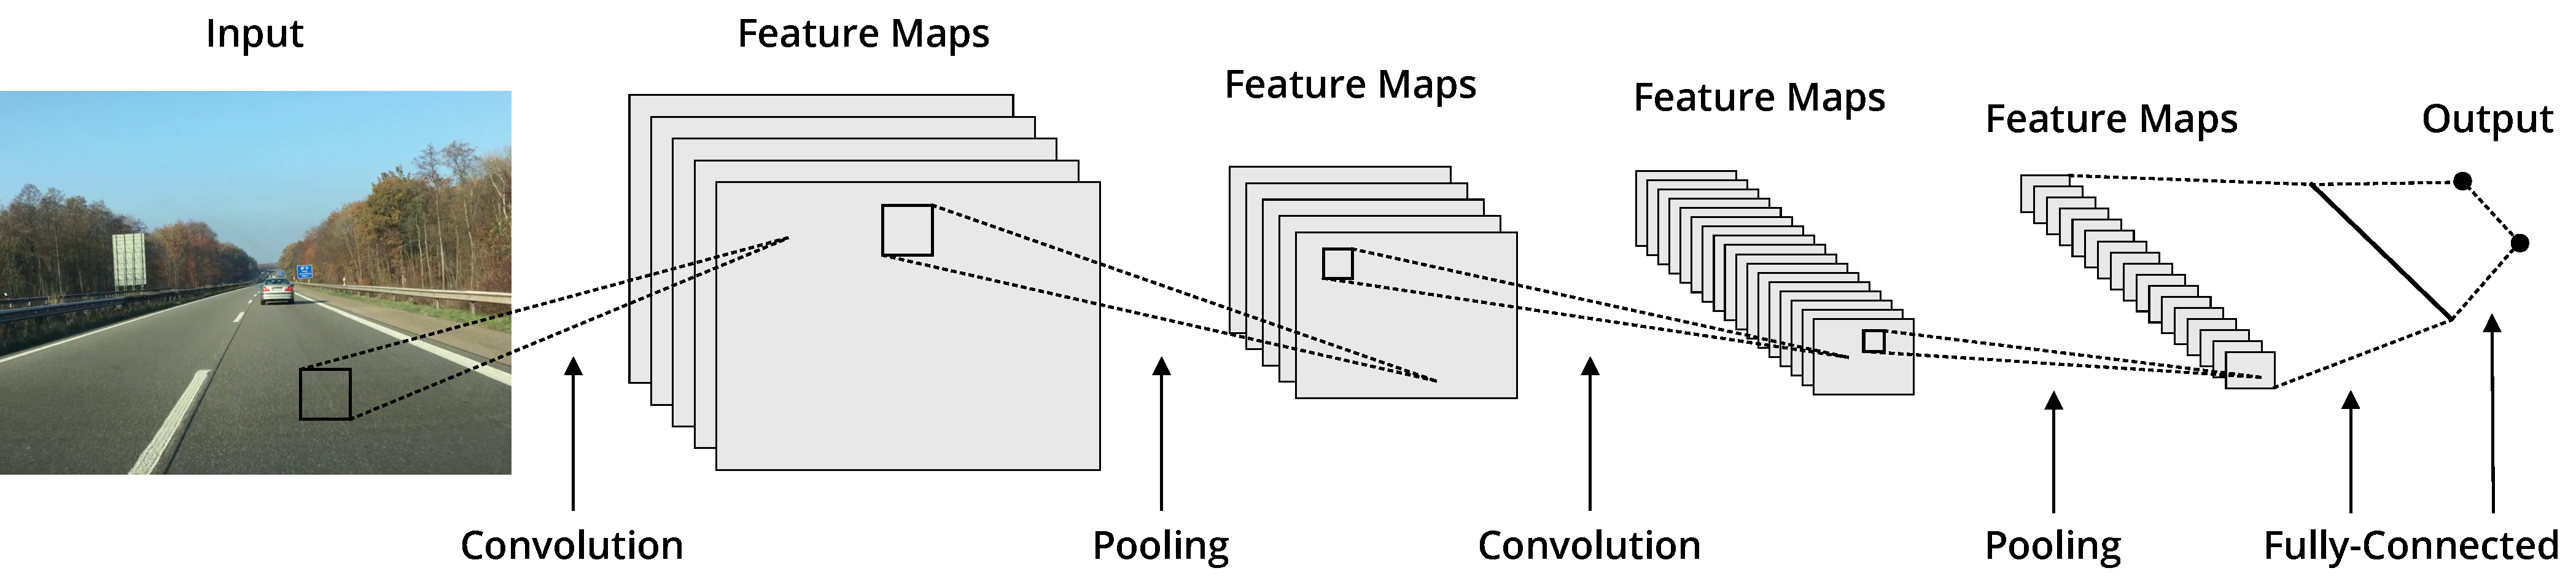
\includegraphics[scale=0.2]{images/cnn.pdf}
\caption{Beispiel eines \aclp{CNN}}
\label{fig_cnn}
\end{figure}


% ===========================
\subsection{Recurrent Neural Networks und LSTMs}
\label{grundlagen_nn_rnn}
% ===========================

In diesem Abschnitt wird die Architektur von \acfp{RNN} und einer modifizierten Version davon, \acfp{LSTM}, vorgestellt. Ein \ac{RNN} ist ein \ac{KNN}, das für sequentielle Daten geeignet ist. Der Unterschied zu der Architektur eines mehrlagigen Perzeptrons ist, dass beim Training auch die Werte von Neuronen derselben Schicht berücksichtigt werden \cite{graves2012rnn}. Damit entsteht nicht nur eine Abhängigkeit zu den Aktivierungswerten der vorherigen Schicht, sondern auch zu den Werten der Neuronen derselben Schicht. Das bedeutet wiederum, dass ein \ac{RNN} nicht von einem einzigen Eingangsvektor abhängig ist, sondern von einer Sequenz von Eingangsvektoren. 

Es gibt verschiedene Architekturen von \acp{RNN}, zum Beispiel mit Ergebniswerten von jedem Input (engl. many to many) oder nur einem Ergebniswert am Ende einer Sequenz (engl. many to one). Die Architekturen mit Ergebniswerten von jedem Input werden beispielsweise für die automatische Übersetzung von Texten verwendet. Dabei ist jeder Input ein neues Wort, für das jeweils ein Ergebnis, wie zum Beispiel eine Übersetzung, produziert wird, und das auch Einfluss auf die Bedeutung der folgenden Wörter hat. Architekturen mit einem Ergebniswert werden für Klassifizierungsprobleme verwendet. Dabei wird einer Sequenz von Inputdaten eine Klasse zugeordnet. Diese beiden Varianten sind beispielhaft in Abbildung \ref{fig_rnn} dargestellt. In dieser Arbeit wird in Kapitel \ref{umsetzung} die Variante mit einem Ergebnis basierend auf einer Sequenz von Inputdaten verwendet, i.e. die Berechnung einer Klasse auf Basis einer Bildsequenz.

\begin{figure}[h]
\centering
\begin{tabular}{c@{\hskip 1cm}c}
\subfloat[many to many]{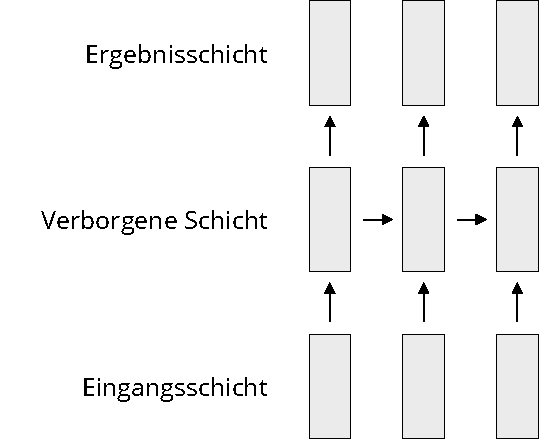
\includegraphics[scale=0.7]{images/rnn_1.pdf}} &
\subfloat[many to one]{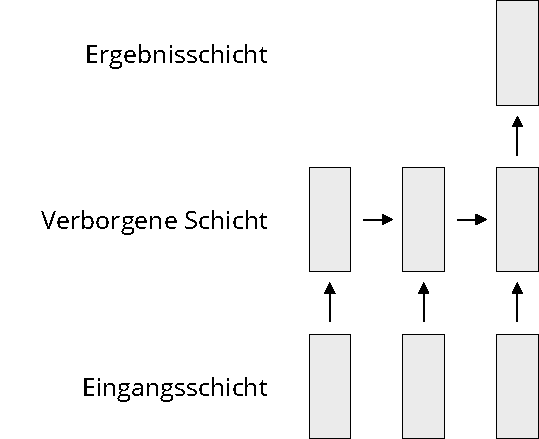
\includegraphics[scale=0.7]{images/rnn_2.pdf}} \\
\end{tabular}
\caption{Beispiel von zwei verschiedenen \ac{RNN}-Architekturen}
\label{fig_rnn}
\end{figure}

Wenn nun in einem \ac{RNN} die Fehlerrückführung (engl. error backpropagation) angewendet wird, kommt es schnell zu dem Problem des verschwindenden oder explodierenden Gradienten (engl. vanishing or exploding gradient). Das basiert auf der Multiplikation der Gradienten von mehreren Sequenzschritten. Wenn der Gradient größer als 1 ist, wächst er sehr stark (explodiert), wenn er kleiner als 1 ist, geht er schnell gegen 0 (verschwindet). In beiden Fällen kann es zu sehr langen Trainingszeiten, in Extremfällen zu keinem Lerneffekt während des Trainings, kommen \cite{graves2012rnn}. Die Lösung dieses Problems wurde von Hochreiter und Schmidhuber \cite{hochreiter1997long} in Form der \ac{LSTM}-Zelle vorgestellt.

Eine \ac{LSTM}-Zelle ist mit drei Toren, dem Eingangstor (engl. input gate), dem Merk- und Vergesstor (engl. forget gate) und dem Ausgangstor (engl. output gate), und einem Zellenzustand aufgebaut. Die Idee ist, dass die \ac{LSTM}-Zelle ein eine Zustand speichern und damit erhalten kann. Das verhindert den Effekt des verschwindenden oder explodierenden Gradienten. Die Abbildung \ref{fig_lstm} zeigt eine solche \ac{LSTM}-Zelle.

\begin{figure}[h]
\centering
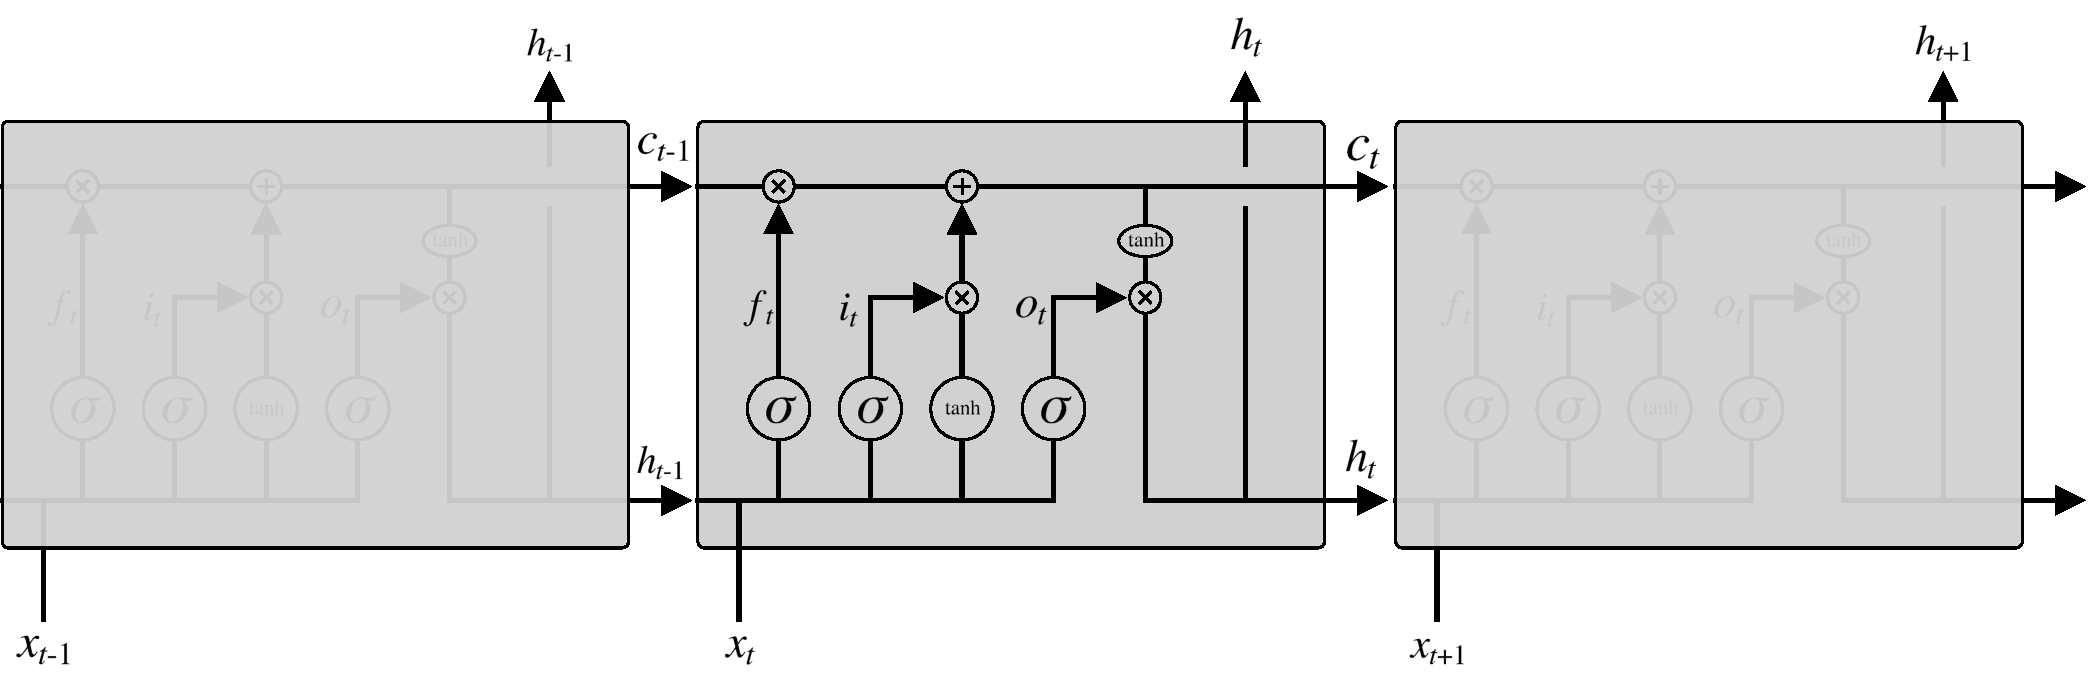
\includegraphics[scale=0.4]{images/lstm.pdf}
\caption[\acl{LSTM}-Zelle]{\acl{LSTM}-Zelle \cite{olah2015lstm}}
\label{fig_lstm}
\end{figure}

Das Vergesstor $f_t$, das Eingangstor $i_t$ und das Ausgangstor $o_t$ ist jeweils mit einer Sigmoid-Funktion $\sigma$ modelliert und hat als Ergebnis einen Wert zwischen 0 und 1. Dieser Wert gibt an, wie durchlässig das jeweilige Tor ist. Der Zustand der Zelle $c_t$ zum Zeitpunkt $t$ wird von der Zelle verwendet, um Werte zu speichern oder zu ändern. $x_t$ ist der Dateninput zum Zeitpunkt $t$. Die Tore $f_t$, $i_t$ und $o_t$, der Zustand der Zelle $c_t$ und der Ergebniswert $h_t$ der Zelle werden mit der jeweiligen Gewichtsmatrix $W$ und dem Bias $b$ wie folgt berechnet \cite{olah2015lstm}.

\begin{equation}
f_t = \sigma (W_f[h_{t-1}, x_t] + b_f)
\end{equation}

\begin{equation}
i_t = \sigma (W_i[h_{t-1}, x_t] + b_i)
\end{equation}

\begin{equation}
o_t = \sigma (W_o[h_{t-1}, x_t] + b_o)
\end{equation}

\begin{equation}
c_t = f_t * c_{t-1} + i_t * \tanh((W_c[h_{t-1}, x_t]) + b_c)
\end{equation}

\begin{equation}
h_t = o_t * \tanh(c_t)
\end{equation}


% ===========================
\subsection{Training mit synthetischen Daten}
\label{grundlagen_nn_synthetisch}
% ===========================

Ein großes Problem beim Training von neuronalen Netzen ist der Aufwand um die Trainings- und Validierungsdaten zu annotieren \cite{richter2016playing}. Ein Ansatz dem entgegenzuwirken ist das Training mit synthetischen Daten oder einer Kombination aus synthetischen und realen Daten. In diesem Abschnitt werden vier Arbeiten aus den letzten Jahren vorgestellt, die diesen Ansatz untersuchen. Diese Arbeiten werden im Abschnitt \ref{umsetzung_daten_real} in Tabelle \ref{tab_datensaetze} zusammengefasst und mit dem Datensatz aus dieser Arbeit verglichen.

Ros et al. \cite{ros2016synthia} haben für die Simulation einer virtuellen Stadt die Unity Development Platform verwendet. Mit virtuellen Fahrten wurden insgesamt circa 200.000 Bilder generiert und diese mit 11 Klassen (e.g. \textit{Sky, Buildings, Road}) auf Pixelebene annotiert. Für das Training wurden die Bilder auf eine Größe von 180 x 120 Pixeln reduziert. Das kombinierte Training mit synthetischen und realen Daten auf den Datensätzen KITTI, CamVid, U-LabelMe und CBCL hat die Genauigkeit (engl. accuracy) auf den realen Testdaten, im Vergleich zum Training mit ausschließlich realen Daten, deutlich gesteigert.

Johnson-Roberson et al. \cite{johnson2017driving} und Richter et al. \cite{richter2016playing} haben für die Generierung von Trainingsdaten das Computerspiel Grand Theft Auto V verwendet. Die Grafikleistung dieses Spiels übertrifft kommerzielle und Open-Source Simulationssoftware und ist daher sehr gut für die Simulation von Bilddaten geeignet. Johnson-Roberson et al. \cite{johnson2017driving} generierten zwei Datensätze mit 50.000 und 200.000 Bildern mit Begrenzungsboxen (engl. bounding boxes) für Fahrzeuge. Mit ihrem kombinierten Training zusammen mit dem KITTI Datensatz konnten sie die Genauigkeit auf den Testdaten, im Vergleich zum Training auf ausschließlich realen Daten, verbessern. Richter et al. \cite{richter2016playing} generierten 25.000 Bilder mit einer Annotation auf Pixelebene von 19 Klassen (e.g. \textit{Road, Sky, Car}). Mit diesen Bildern und einem kombinierten Training zusammen mit dem KITTI Datensatz konnten auch sie die Genauigkeit verbessern.

Tremblay et al. \cite{tremblay2018training} verfolgten bei der Generierung von Bildern einen etwas anderen Ansatz. Sie nutzten 3D Modelle von Fahrzeugen und platzierten diese mit zufällige Positionen und Ausrichtungen auf verschiedene reale Szenen. Die 100.000 Bilder wurden mit Begrenzungsboxen (engl. bounding boxes) um Fahrzeuge annotiert. Beim Training wurden ausschließlich die synthetischen Daten verwendet und es wurde eine Genauigkeit von circa 80 Prozent erreicht.

Generell zeigt das Training von neuronalen Netzen mit einer Kombination von synthetischen und realen Daten bereits vielversprechende Ergebnisse, auf denen dieses Arbeit aufbauen will. Im Gegensatz zu den vergangenen Arbeiten, werden in dieser Arbeit ganze Szenarien generiert und annotiert und nicht einzelne Bilder mit Begrenzungsboxen oder semantischer Annotation auf Pixelebene.


% ===========================
\subsection{Klassifizierung von Videos}
\label{grundlagen_nn_video}
% ===========================

Grundsätzlich kann zwischen drei verschiedenen Ansätzen bei der Klassifizierung von Videos mit \acp{KNN} unterschieden werden. Beim ersten Ansatz werden die einzelnen Bilder aus einem Video mit einem \ac{CNN} klassifiziert und anschließend wird das Video der Klasse zugeordnet, zu der die meisten Bilder zugeordnet wurden \cite{karpathy2014large}. Mit diesem Ansatz werden die räumlichen Merkmale (engl. spatial features) mit dem \ac{CNN} sehr gut extrahiert und bei der Klassifizierung berücksichtigt. Das Problem ist, dass zeitliche Merkmale (engl. temporal features) keine Beachtung finden und die Reihenfolge der einzelnen Bilder ignoriert wird. Dieser Ansatz ist in Abbildung \ref{fig_single_frame_classification} dargestellt.

\begin{figure}[h]
\centering
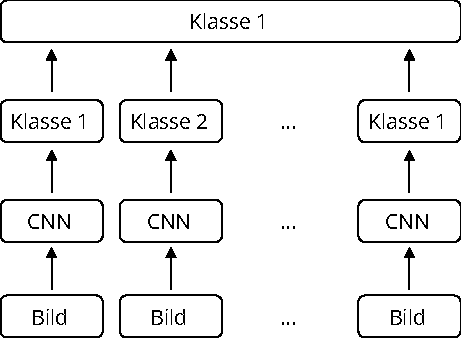
\includegraphics[scale=0.8]{images/single_frame_classification.pdf}
\caption{Klassifizierung von einzelnen Bildern mit anschließender Klassifizierung des gesamten Videos}
\label{fig_single_frame_classification}
\end{figure}

Ein weiterer Ansatz basiert auf der Idee, Feature Maps von mehreren Bildern zu kombinieren und damit die zeitlichen Merkmalen mit 3D-Filtern eines \acp{CNN} zu extrahieren. In früheren Arbeiten dazu wurde für diese Kombination eine Pooling-Operation verwendet \cite{karpathy2014large, yue2015beyond} und es wurden verschiedene Architekturen mit früher, später oder langsamer Fusion verwendet (engl. early, late, and slow fusion). Bei der frühen Fusion werden schon zu Beginn die Eingangswerte von mehreren Bildern kombiniert und dann zusammen die Feature Maps berechnet. Bei der späten Fusion werden von allen Bildern einzeln die Merkmale extrahiert und erst am Ende mit einer Pooling-Schicht vereint. Beim Ansatz der langsamen Fusion werden schrittweise die Feature Maps von immer mehr Bildern zusammengefasst. Diese Architekturen sind schematisch in Abbildung \ref{fig_fusion_classification} dargestellt.

\begin{figure}[h]
\centering
\begin{tabular}{c@{\hskip 0.7cm}c@{\hskip 0.7cm}c}
\subfloat[Frühe Fusion]{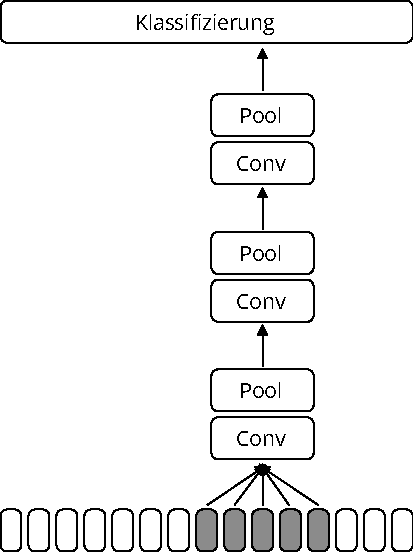
\includegraphics[scale=0.6]{images/fusion_early.pdf}} &
\subfloat[Späte Fusion]{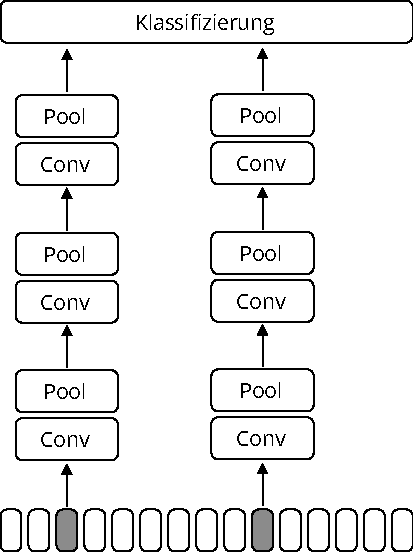
\includegraphics[scale=0.6]{images/fusion_late.pdf}} &
\subfloat[Langsame Fusion]{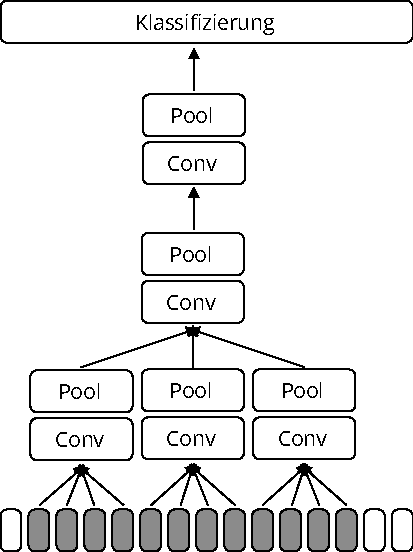
\includegraphics[scale=0.6]{images/fusion_slow.pdf}} 
\end{tabular}
\caption[Schematische Darstellung von Klassifizierungsarchitekturen mit frühen, späten und langsamen Fusionen von Feature Maps]{Schematische Darstellung von Klassifizierungsarchitekturen mit frühen, späten und langsamen Fusionen von Feature Maps \cite{karpathy2014large}}
\label{fig_fusion_classification}
\end{figure}

Später wurden neben der Pooling-Operation andere Operationen für die Fusion entwickelt \cite{feichtenhofer2016convolutional}. Obwohl damit teilweise sehr gute Ergebnisse erzielt werden konnten \cite{carreira2017quo}, haben die Fusions-Architekturen einen entscheidenden Nachteil. Zeitliche Merkmale werden berücksichtigt, allerdings nicht die Reihenfolge der Bilder. Aus diesem Grund gibt es einen dritten Ansatz für die Klassifizierung von Videos, die Kombination aus \acp{CNN}, die räumliche Merkmale extrahieren, und \acp{LSTM}, die zeitliche Merkmale extrahieren. Eine Architektur mit diesem Ansatz wurde von Donahue et al. \cite{donahue2015long} vorgestellt. Dabei wird ein vortrainiertes \ac{CNN} verwendet, um die räumlichen Merkmale aus allen Bildern zu extrahieren. Anschließend werden diese Feature Maps einer \ac{LSTM}-Schicht übergeben, welche die zeitlichen Merkmale extrahiert. In Abbildung \ref{fig_cnn_lstm_architektur} ist diese Architektur schematisch dargestellt.

\begin{figure}[h]
\centering
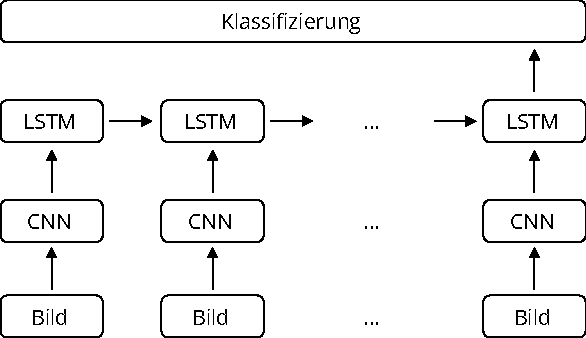
\includegraphics[scale=0.8]{images/cnn_lstm_architektur.pdf}
\caption[Klassifizierung von Videos mit einer \ac{CNN}-\ac{LSTM}-Architektur]{Klassifizierung von Videos mit einer \ac{CNN}-\ac{LSTM}-Architektur \cite{donahue2015long}}
\label{fig_cnn_lstm_architektur}
\end{figure}

In dieser Arbeit wird der erste Ansatz, die Klassifizierung von einzelnen Bilder mit anschließender Klassifizierung des gesamten Videos, und der dritte Ansatz, die kombinierte \ac{CNN}-\ac{LSTM}-Architektur verwendet. Die Architekturen dieser Arbeit werden im Detail in Abschnitt \ref{umsetzung_training_architektur} vorgestellt.

